\documentclass[final]{fhnwreport}         %[mode] = draft or final
%%---Main Packages-----------------------------------------------------------------------
\usepackage[english, ngerman]{babel}	%Mul­tilin­gual sup­port for LaTeX
\addto\extrasngerman{%
  \renewcommand{\sectionautorefname}{Abschnitt}%
  \renewcommand{\subsectionautorefname}{Unterabschnitt}%
  \renewcommand{\subsubsectionautorefname}{Unterunterabschnitt}%
  \renewcommand{\tableautorefname}{Tabelle}%
}
\usepackage[T1]{fontenc}				      %Stan­dard pack­age for se­lect­ing font en­cod­ings
\usepackage[utf8]{inputenc}				  %Ac­cept dif­fer­ent in­put en­cod­ings
\usepackage{lmodern}                 %The newer Font-Set
\usepackage{textcomp}					      %LaTeX sup­port for the Text Com­pan­ion fonts
\usepackage{graphicx} 					      %En­hanced sup­port for graph­ics
\usepackage{svg}
\usepackage{float}						        %Im­proved in­ter­face for float­ing ob­jects
%\usepackage{ifdraft}                %Let you check if the doc is in draft mode

%%---Useful Packages---------------------------------------------------------------------
% \usepackage[pdftex,dvipsnames]{xcolor}  %Driver-in­de­pen­dent color ex­ten­sions for LaTeX
\usepackage{csquotes}                   %Simpler quoting with \enquote{}
\usepackage{siunitx} 					     %A com­pre­hen­sive (SI) units pack­age
\usepackage{listings}					     %Type­set source code list­ings us­ing LaTeX
\lstset{
  basicstyle=\ttfamily\small,
  breaklines=true,
  breakatwhitespace=false,  % allow breaking inside long tokens (URLs, keys, etc.)
  columns=fullflexible,      % let listings adjust character widths to enable breaks
  keepspaces=true,
  showstringspaces=false,
  tabsize=2,
  % optional: visual cue for wrapped lines
  postbreak=\mbox{\textcolor{gray}{$\hookrightarrow$}\space}
}
\usepackage[bottom]{footmisc}			  %A range of foot­note op­tions
\usepackage{footnote}					     %Im­prove on LaTeX's foot­note han­dling
\usepackage{verbatim}					     %Reim­ple­men­ta­tion of and ex­ten­sions to LaTeX ver­ba­tim
\usepackage[textsize=footnotesize]{todonotes} %Mark­ing things to do in a LaTeX doc­u­ment
\usepackage{lipsum}              % Gives you access to blindtext
\usepackage[acronym]{glossaries}
\makeglossaries 
\usepackage{pgfgantt}
\hypersetup{colorlinks=true, urlcolor=blue, linkcolor=black, citecolor=blue}
\usepackage{soul}
\usepackage{msc} % For sequence diagrams
\usepackage{makecell}
\usepackage{changepage}
%%---Tikz Packages-----------------------------------------------------------------------
%\usepackage{standalone}
\usepackage{tikz}
\usetikzlibrary{shapes.geometric, arrows.meta, positioning}
\tikzstyle{block} = [
    rectangle,
    rounded corners,
    minimum height=1.2cm,
    % minimum width=3cm,
    text centered,
    draw=black,
    fill=blue!20,
    align=center
]
\tikzstyle{arrow} = [thick,->,>=stealth]
% \usepackage{tikz-uml}
\usetikzlibrary{shapes.geometric, arrows.meta, positioning}
%\usepackage{circuitikz}
%\usetikzlibrary{arrows}
%\usetikzlibrary{calc}
%\usetikzlibrary{intersections}

%%---Math Packages-----------------------------------------------------------------------
\usepackage{amsmath}					    %AMS math­e­mat­i­cal fa­cil­i­ties for LaTeX
%\usepackage{amssymb}					  %Type­set­ting symbols (AMS style)
\usepackage{ragged2e,array}						  %Ex­tend­ing the ar­ray and tab­u­lar en­vi­ron­ments
\newcolumntype{Y}{>{\RaggedRight\arraybackslash}X} % ragged-right wrapping
%\usepackage{amsthm}					    %Type­set­ting the­o­rems (AMS style)

%%---Table Packages----------------------------------------------------------------------
\usepackage{tabularx}					  %Tab­u­lars with ad­justable-width columns
%\usepackage{longtable}
\usepackage{ltablex}   % combines longtable + tabularx
\keepXColumns   
\usepackage{multirow}					  %Create tab­u­lar cells span­ning mul­ti­ple rows
\usepackage{multicol}					  %In­ter­mix sin­gle and mul­ti­ple columns

%%---PDF / Figure Packages---------------------------------------------------------------
\usepackage{pdfpages}					  %In­clude PDF doc­u­ments in LaTeX
\usepackage{pdflscape}					  %Make land­scape pages dis­play as land­scape
%\usepackage{subfig}					    %Fig­ures di­vided into sub­fig­ures

%%---Other Packages----------------------------------------------------------------------
%\usepackage{xargs}              %De­fine com­mands with many op­tional ar­gu­ments
%\usepackage{drawio}              %In­clude draw.io di­a­grams di­rectly in LaTeX

%%---Main Settings-----------------------------------------------------------------------
\graphicspath{{./graphics/}}			%Defines the graphicspath
%\geometry{twoside=false}				%twoside=false disables the "bookstyle"
\setlength{\marginparwidth}{2cm}
\overfullrule=5em						    %Creates a black rule if text goes over the margins => debugging

%%---User Definitions--------------------------------------------------------------------
%%Tabel-Definitions: (requires \usepackage{tabularx})
\newcolumntype{L}[1]{>{\raggedright\arraybackslash\sloppy\hspace{0pt}}p{#1}}    %column-width and alignment
\newcolumntype{C}[1]{>{\centering\arraybackslash}p{#1}}
\newcolumntype{R}[1]{>{\raggedleft\arraybackslash}p{#1}}					

% \newcommand{\ac}[1]{\gls{#1}}
\newcommand{\ac}[1]{%
  \ifglsused{#1}%
    {\gls{#1}\textsuperscript{*}}% If already used → add asterisk
    {\gls{#1}}% If first time → no asterisk
}
% Set caption labels for figures and their references
\renewcaptionname{ngerman}{\figurename}{Abbildung}
\addto\extrasngerman{\renewcommand{\figureautorefname}{Abbildung}}

% Command for referencing sections with number and name
% \newcommand*{\fullref}[1]{\hyperref[{#1}]{\ref*{#1} \nameref*{#1}}}
\newcommand*{\fullref}[1]{%
  \autoref{#1} (\nameref{#1})%
}                        %loads all packages, definitions and settings	
\newacronym{CSB}{CSB}{Cloud Service Broker}
\newacronym{bv}{BV}{Bundesverwaltung}
\newacronym{bit}{BIT}{Bundesamt für Informatik und Telekommunikation}
\newacronym{sgc}{SGC}{Swiss Government Cloud}
\newacronym{oscal}{OSCAL}{Open Security Controls und Assessment Language}
\newacronym{owl}{OWL}{Web Ontology Languge}
\newacronym{pvp}{PVP}{Policy Validation Points}
\newacronym{sspm}{SSPM}{System Security Plan Model}
\newacronym{ap}{AP}{Assessment Plan}
\newacronym{apr}{APR}{Assessment Plan Result}
\newacronym{compd}{Component Definitions}{Component Definitions}
\newacronym{iac}{IaC}{Infrastructure as Code}
\newacronym{si001}{Si001}{Si001 - IKT Grundschutz der Bundesverwaltung}
\newacronym{tosca}{TOSCA}{Topology and Orchestration Specification for Cloud Applications}
\newacronym{occi}{OCCI}{Open Cloud Computing Interface}
\newacronym{dsl}{DSL}{domain specific language}
\newacronym{poc}{PoC}{Proof of concept}
\newacronym{nist}{NIST}{National Institute of Standards and Technology}
\newacronym{rdf}{RDF}{Resource Description Framework}
\newacronym{vm}{VM}{virtual Machine}
\newacronym{k8s}{K8s}{Kubernetes}
\newacronym{aws}{AWS}{Amazon Web Services}
\newacronym{osco}{OSCO}{Openshift Compliance Operator}
\newacronym{scap}{SCAP}{Security Content Automation Protocol}
\newacronym{cac}{CAC}{Compliance Administration Center}
\newacronym{gcp}{GCP}{Google Cloud Platform}
\newacronym{nfr}{NFR}{Non-Functional Requirements}
\newacronym{tshirt}{T-Shirt-Size}{T-Shirt-Size S, M, L, XL}
\newacronym{uc}{UC}{Use-Case}
\newacronym{cli}{CLI}{Command Line Interface}
\newacronym{sdk}{SDK}{Software Development Kit}
\newacronym{aks}{AKS}{Azure Kubernetes Service}
\newacronym{cis}{CIS}{Center for Internet Security}
\newacronym{ki}{KI}{Künstliche Intelligenz}
\newacronym{ctrl}{Control}{\ac{oscal} Control}
\newacronym{lz}{LZ}{Landing Zone}
\newacronym{llm}{LLM}{Large Language Model}
\newacronym{ea}{EA}{Enterprise-Architecture}
\newacronym{togaf}{TOGAF}{The Open Group Architecture Framework}
\newacronym{adm}{ADM}{Architecture Development Method}
\newacronym{bdat}{B-D-A-T}{Business,Data,Application,Technology}
\newacronym{mvp}{MVP}{Minimum Viable Product}
\newacronym{iam}{IAM}{Identity and Accessmanagement}

%%%%% Logo: Hocvhschule HTU oder HSI, Sprache DE oder EN:
%\newcommand{\logofilename}{FHNW_HTU_DE}
%\newcommand{\logofilename}{FHNW_HTU_EN}
\newcommand{\logofilename}{FHNW_HSI_DE}
%\newcommand{\logofilename}{FHNW_HSI_EN}
%%%%%
%%%%% Bibliographie entweder im IEEE- oder im APA-Stil:
%\usepackage[style=ieee,urldate=comp,backend=biber]{biblatex}
\usepackage[style=apa,urldate=comp,backend=biber,bibencoding=utf8]{biblatex}
%%%%%
% \addbibresource{literature/bib.bib}
\addbibresource{literature/zotero.bib}

\title{Enterprise-Architektur von multicloud-konformen Landingzones}  %Project Title
\author{Bachelorthesis}    %Document Type => Technical Report, ...
\date{Windisch, September 2025}               %Place and Date

\begin{document}

\pagenumbering{roman}	

%%---TITLEPAGE---------------------------------------------------------------------------
\selectlanguage{ngerman}                  %ngerman or english
\maketitle

\vfill

\begin{figure}[H]
\centering
\includegraphics[width=\linewidth]{bitcloud2.png}
\end{figure}

\vfill

\begin{tabular}{@{}p{5cm} l}
Studentin/Student          &    Frithjof Hoppe\\
                           &    Benjamin Dätwyler\\[2ex]
Expertin/Experte           &    Romano Rot\\[2ex]
Fachbetreuer/in            &    Sebastian Graf\\[2ex]
Auftraggeber               &    Sebastian Matyas\\[2ex]
                           &    Thierry Perroud\\[2ex]
Projektnummer              &    25HS\_IMVS17\\[4ex]
\multicolumn{2}{@{}l}{Fachhochschule Nordwestschweiz, Hochschule für Informatik}
\end{tabular}

\vspace*{4ex}
% Logo Industriepartner
\begin{tikzpicture}[remember picture,overlay,every node/.style={anchor=north east}]
  \node at (current page.north east) [xshift=-1cm, yshift=-1cm] {
\includegraphics[width=8cm]{BIT_d_rgb_pos_quer_pf.jpg}};
\end{tikzpicture}

\clearpage

%%---ABSTRACT----------------------------------------------------------------------------
\selectlanguage{ngerman}				%ngerman or english
\thispagestyle{empty}
\section*{Abstract}
\hl{TODO Abstract}

\vspace{2ex}

\textbf{Keywords:}

\hl{TODO keywords}

% \clearpage

% \section*{Vorwort / Dank}

% \hl{TODO vorwort}



%%---TABLE OF CONTENTS-------------------------------------------------------------------	
\selectlanguage{ngerman}				%ngerman or english
\tableofcontents
\clearpage

\listoffigures
\listoftables
\cleardoublepage

%%---TEXT--------------------------------------------------------------------------------

\pagenumbering{arabic}
\section{Introduction}
\label{sec:introduction}


1.1 Background
•	Increasing relevance of cloud governance in multi-cloud and hybrid-cloud environments 
•	Use of the term landing zone by major cloud providers such as Azure, AWS, GCP, Alibaba Cloud, and IBM Cloud 
•	Importance of structured foundational environments for secure and manageable cloud adoption 
1.2 Problem Statement
•	The concept of a landing zone is not defined uniformly across providers 
•	Differences in terminology, structure, and emphasis make direct comparison difficult 
•	A comparative understanding is needed to clarify the concept in a technical context 
1.3 Aim of the Report
•	To analyze how major cloud providers define and structure landing zones 
•	To identify the main similarities and differences between provider concepts 
•	To formulate a common definition based on the comparison 
1.4 Research Question
•	How do landing zone concepts differ across major cloud providers, and what common definition can be derived from their similarities and differences? 
1.5 Scope and Limitations
•	Focus on conceptual comparison rather than implementation details 
•	Focus on selected providers: Azure, AWS, GCP, Alibaba Cloud, and IBM Cloud 
•	Focus on landing zones as foundational structures for governance, security, and workload enablement 
•	Limitation to publicly available provider documentation and selected technical literature 
1.6 Structure of the Report
•	Chapter 1 introduces the topic, problem, objective, and scope 
•	Chapter 2 reviews the conceptual and technical background 
•	Chapter 3 presents the methodology and comparison framework 
•	Chapter 4 provides the comparative analysis and synthesis 
•	Chapter 5 discusses the significance and limitations of the findings 
•	Chapter 6 concludes the report by answering the research question and summarizing the main outcome 

% \section{Ausgangslage}

Die Bundesverwaltung verfolgt eine Hybrid-Multi-Cloud Strategie, welche die Nutzung unterschiedlicher Cloud-Anbieter sowie der eigenen Infrastrukturen kombiniert. Das Bundesamt für Informatik und Telekommunikation (BIT) nimmt dabei die Rolle eines Cloud Service Brokers (CSB) wahr: Es stellt die Anbindung an verschiedene Hyperscaler sicher und betreibt gleichzeitig eine eigene On-Premises-Infrastruktur.

Für den Betrieb von Cloud-Diensten nutzen die einzelnen Provider sogenannte Landingzones - vordefinierte Strukturen, die den Rahmen für die Nutzung der jeweiligen Plattform bilden. Die bisherigen Erfahrungen zeigen jedoch, dass sich diese Landingzones zwischen den Anbietern grundlegend unterscheiden und bisher keine übergreifende technische Lösung existiert, die eine einheitliche Nutzung und Steuerung über mehrere Plattformen hinweg ermöglicht.

Damit entsteht die Herausforderung, Anforderungen und zentrale Elemente einer Provider-agnostischen Landingzone zu identifizieren, die eine konsistente, sichere und Compliance-konforme Nutzung der verschiedenen Plattformen innerhalb der Bundesverwaltung sicherstellt.

Im Rahmen des IP5 Projektes \textit{25fs imvs29} wurde sich zudem bereits mit der plattformübergreifenden Governance auseinandergesetzt. Mit einem PoC wurde dort gezeigt, dass eine agnostische Implementation grundsätzlich möglich ist. Die Erkenntnisse daraus haben möglicherweise Implikationen auf Teilaspekte der Arbeit in dieser Bachelorthesis.
% \section{Problemstellung}

Eine Nutzung der verschiedenen Cloud-Plattformen bedingt, dass eine grundlegende Struktur existiert auf welche Anwender der Bundesverwaltung aufbauen können. Das BIT verwendet hierfür den etablierten Begriff der Landingzone.

Als Landingzone wird eine durch den Plattformprovider vordefinierten Struktur bezeichnet, in welcher die effektiven Angebote bezogen werden können.

Aus der bisherigen Erfahrung unterschieden sich die Plattformprovider in der Art und Weise wie ihre Plattform konzeptioniert ist. Die Problemstellung ist somit, dass die Plattformen zwar verschieden sind, jedoch im Idealfall homogenisiert werden müssten. Eine Vereinheitlichung ermöglicht es dem BIT einen Leitrahmen zu definieren welcher für die verschiedenen Projekte gilt, welche ihre Vorhaben auf der Plattform laufen lassen.
\section{Grundlagen und Stand der Technik}
\label{sec:grundlagen}

% \hl{structure notes start}
% \begin{itemize}
%     \item Aufzeigen dass es die Idee der Landing Zone bereits auf verschiedenen Plattformen gibt
%     \item Vergleich der verschiedenen Landing Zone Aspekte von den bekannten Cloud-Providern → Tabelle welche bereits im Vorhinein erstellt wurde
%     \item Kriterien aus bestehenden Arbeiten welche als Basis für Evaluationskriterien dienen können → Quasi aufzeigen dass die Kriterien welche wir definiert haben fundiert sind. Kriteren können zwar BIT/BV spezifische Sachen beinhalten sollten jedoch auch gewissermassen \flqq neutral\frqq\ sein
% \end{itemize}
% \hl{structure notes end}

Die Nutzung vom Begriff \ac{lz} selbst beschränkt sich in theoretischer Literatur mehrheitlich auf Referenzen von Cloud-Plattformen selbst und wird nicht explizit aufgegriffen. Ebenso finden sich keine ausführlichen Konzepte, wie \ac{lz} selbst zu strukturieren sind. In der Praxis bei den Cloud-Plattformen hingegen existiert ein genaueres Verständnis worum es sich bei einer \ac{lz} handelt. So wird sie nach \cite{microsoft_what_2025} bspw. bezeichnet als Möglichkeit zum Einrichten / Verwalten der Kundenumgebung mit dem Ziel eine Konsistenz bezüglich Sicherheit, Compliance, Betriebseffizienz etc. zu erhalten. Dieses Ziel kann als einer der treibenden Faktoren betrachtet werden, warum \ac{lz} relevant sind. Reduziert kann gesagt werden, dass durch eine \ac{lz} die Cloud-Plattformen als solche verfügbar und vor allem auf eine sichere Art nutzbar für eine Organisation gemacht wird \parencite[Kapitel 6]{mulder_multi-cloud_2020}. Eine sichere Nutzung bedingt zuerst dass die Veranwortlichkeiten zwischen Cloud-Plattform und dem Nutzer klar sind. Mit dem Modell der geteilten Verantwortung (oder auch Shared Responsibility Model) zeigen Plattformen deshalb auf, welchen Teil der Sicherung vom Kunden oder durch die Cloud-Plattform selbst erbracht werden müssen \parencite{aws_cloud_security_modell_nodate}. Für eine Organisationen heisst dies häufig, dass man sich bewusst werden muss welche Anforderungen man selbst hat. Diese können bspw. regulatorisch aus Dokumenten wie \ac{si001} wie auch organisatorisch durch Expertenteams / Plattformteams begründet sein. Die Themen welche relvant sind ähneln sich dabei über die Cloud-Plattformen hinweg. \ac{iam}, Network, Security sind dabei nur einige Beispiele.

Trotz der Gemeinsamkeiten dass eine Governance als notwendig verstanden wird, weisen die Cloud-Plattformen jedoch auch Unterschiede auf. Diese erstrecken sich von eigenen Metamodellen bis zu unterschiedlichen Implementation von Komponenten. Eine Organisation welche eine sichere Nutzung im multi-cloud Kontext sicherstellen möchte steht somit vor der Herausforderung, wie es die verschiedenen Cloud-Plattformen verwaltet. Hierfür existieren auf dem Markt bereits diverse Cloud Management Plattformen (bspw Flexera One, Cloud Bolt, HPE Morpheus), welche sich haupsächliche auf die operative Verwaltung und Bereitstellung von Cloud-Ressourcen spezialisieren. In anderen Worten wird addressiert wie die konkrete Implementation in einem multi-cloud Setup möglich ist. Offener dagegen ist wie die Strukturierung der Cloud-Ressourcen aussieht und welche Policies warum einer Cloud-Ressource zugewiesen werden müssen. Die Komplexität dieser Governance versuchen Cloud-Plattformen zwar individuell zu lösen, womit aber ein allgemeiner Ansatz fehlt. Diese Arbeit fokussiert sich deshalb auf einen Abstraktionsansatz für Governacne und nicht einer weiteren Cloud Management Plattform.

Für einen Abstraktionsansatz sind hierbei konkte die Security Frameworks relevant, dess Compliance sichergestellt werden soll. Ein prominentes Beispiel für die \ac{bv} ist \ac{si001}, welcher den IKT Grundschutz der \ac{bv} beschreibt. Ein anderes bekanntes Framework ist die \ac{nist} Special Publication 800-53. Beide genannten Regulation weisen mit Controls eine im Kern gleiche Struktur auf. Wichtiger jedoch ist, dass die korrekte Anwendung der Regulationen für Organisationen welche sie nutzen indirekt ein Ziel darstellt. Die Motvation kann dabei unterschiedlich sein (gesetztliche Vorgaben, selbstauferlegt etc.).

% start chat gpt
Mit den Regulation als Beispel stellt sich die Frage auf welcher Ebene eine solche Governance-Strukturierung erfolgen kann. Da Anforderungen aus regulatorischen Vorgaben oder organisationalen Zielsetzungen letztlich durch technische Architekturentscheidungen umgesetzt werden müssen, kann die Gestaltung von Landing Zones als ein architektonisches Problem verstanden werden.

Insbesondere im Multi-Cloud-Kontext entsteht dadurch die Notwendigkeit, eine Abstraktionsebene zu finden, welche unabhängig von spezifischen Implementationen einzelner Cloud-Provider funktioniert. Eine mögliche Perspektive hierfür bietet die Betrachtung von Fähigkeiten (\textit{Capabilities}) einer Organisation. Capabilities beschreiben stabilere, technologieunabhängige Möglichkeiten zur Erbringung bestimmter Leistungen, wie etwa das Management von Identitäten, die Segmentierung von Netzwerken oder die Überwachung von Systemzuständen.

Im Kontext von Enterprise-Architecture-Frameworks dienen Capabilities häufig als strukturierendes Element, um strategische Anforderungen mit konkreten Architekturartefakten in Beziehung zu setzen. Dadurch entsteht eine Grundlage, um Governance-Mechanismen wie Policies oder Controls systematisch einzuordnen und deren Umsetzung nachvollziehbar zu gestalten.
% end chat gpt

\section{Methodik und Vorgehen}
\label{sec:methodik}

\subsection{Forschungsmethodischer Ansatz}
\label{sec:methodik-intro}
\hl{stucture start}
\begin{itemize}
    \item Annahmen aufzeigen auf welchen die Arbeit aufbaut
    \item Strukturierung des Vorgehen gem Drawio Prozess → Grundlage basierend auf Enterprise Architektur-Buch. Quasi von Business hinzu Anforderungen kommen, deshalb haben wir das mittel der capability map gewählt etc.
\end{itemize}
\hl{structure end}

\subsection{Vorgehen zur Identifikation von Landingzone Komponenten}
\label{sec:methodik-landingzones}
\hl{stucture start}
\begin{itemize}
    \item Kriterien beschreiben mit welchen die verschiedenen Provider analysiert wurden, bspw Aspekte und so
    \item Detaillierte Beschreibung der Erkenntnis bzw Tabelle
\end{itemize}
\hl{structure end}

\subsection{Synthese eines abstrahierten Metamodells}
\label{sec:methodik-metamodell}
\hl{stucture start}
\begin{itemize}
    \item Metamodell definieren basierend auf Fachbegriffen und Domänenbegriffen
\end{itemize}
\hl{structure end}

\subsection{Erhebung von Landing-Zone Fähigkeiten}
\label{sec:methodik-capability}
\hl{stucture start}
\begin{itemize}
    \item Quasi als Folge → Erstellen Capability Map inkl Auswahl durch den Auftraggeber (Iteration mit L1/L2 Strukturierung)
    \item Priorisierung der Capabilities mit Auftraggeber
\end{itemize}
\hl{structure end}

\subsection{Strukturierung der Evaluation der Architektur}
\label{sec:methodik-evaluation}
\hl{stucture start}
\begin{itemize}
    \item Evaluationskriterien für Traceability Architektur definieren
    \item Use-Cases definieren / Ausprägung
\end{itemize}
\hl{structure end}


\subsection{Strukturierung der Evaluation der Architektur}
\label{sec:methodik-evaluation}

Damit über die Einordnung der Traceability-Architektur selbst und den Varianten der Traceabilityarchitektur aus \fullref{sec:traceability-architecture} eine Aussage ob einer optimalen Architektur (im Sinne der leitenden Fragestellung) gemacht werden kann ist folgende Methodik vorgesehen:

\begin{enumerate}
    \item Identifikation relevanter Bewertungsdimensionen für die Architektur selbst wie die Varianten
    \item Recherche und Ableitung von Kriterien innerhalb der Bewertungsdimensionen (sowohl vom \ac{bit} als auch aus der Literatur)
    \item Ableitung eines Konformitätschecks der Traceability-Architektur an sich
    \item Ableitung Bewertungsprozesses für die Traceability-Architektur Varianten
    
\end{enumerate}

Basierend auf der Orientierung an \ac{togaf} wird sich bei der Suche an Dimensionen an dem \ac{adm} Cycle orientiert. Folgende Dimensionen werden ausgewählt:

\begin{longtable}{|
  L{3cm}|
  p{\dimexpr(\textwidth-3cm-6\tabcolsep-4\arrayrulewidth)/2\relax}|
  p{\dimexpr(\textwidth-3cm-6\tabcolsep-4\arrayrulewidth)/2\relax}|
}
    \hline
    \textbf{Dimension} & \textbf{Beschreibung} & \textbf{Begründung} \\
    \hline
    \endfirsthead

    \hline
    \textbf{Dimension} & \textbf{Beschreibung} & \textbf{Begründung} \\
    \hline
    \endhead

    Architekturprinzipien &
    Prinzipien oder grundlegende Eigenschaften einer Architektur. Architekturprinzipien können eingehalten oder nicht eingehalten sein. Dies ist eine Evaluationsdimension, welche auf die Traceability-Architektur als angewendet wird &
    Ergeben sich aus der Preliminary Phase im \ac{adm} Cycle in welcher die allg. Rahmenbedingungen gesetzt werden, von der Architekturprinzipien teil sind. Die Architekturprinzipien sind als Gatekeeper für Varianten gedacht
    \\
    \hline
    Qualitätsmerkmale &
    Qualitative Eigenschaften der Architektur analog zu klassischen \ac{nfr}. Qualitätsmerkmale können basierend auf einer Skala zu einem gewissen Mass erfüllt sein. Dies ist eine Evaluationsdimension, welche auf die verschiedenen Varianten der Architektur angewendet wird &
    Ergeben sich gedanklich aus den Phasen A-D im \ac{adm} Cycle und dienen als vergleichende Kriterien zwischen verschiedenen Varianten
    \\
    \hline
    Entscheidung und Trade-Off &
    Spannungsfelder unterschiedlicher Architekturrichtungen welche nicht per se richtig oder falsch sind. Trade-Off Kriterien werden zum Labeling / zur Charakterisierung verwendet. Dies ist eine Evaluationsdimension, welche auf die verschiedenen Varianten der Architektur angewendet wird &
    Ergibt sich gedanklich aus den Phasen E-F im \ac{adm} Cycle. Sollen die Eigenschaften der unterschiedlichen Varianten hervorheben, ohne wertend zu wirken, da die durch das Kriterium vergleichenden Eigenschaften  grundsätzlich keine negative/positive Konnotation besitzen sollen
    \\
    \hline
    Kontext und Anwendung &
    Konkrete Rahmenbedingungen aus dem \ac{bit} Use-Case, welche den Bewertungskontext der Evaluationskriterien bzw. Evaluationsdimensionen beeinflusst. &
    Ergibt sich aus der Festlegung des Kontextes in der Preliminary Phase und Ausarbeitung in den Phasen B-D im \ac{adm} Cycle. Dient dazu im Rahmen des definierten Use-Cases zu beurteilen. Im Gegensatz zu den Architekturprinzipien des \ac{bit} ist der Use-Case flexibler
    \\
    \hline
    \caption{Identifizierte Dimensionen des Evaluationsframeworks}
    \label{tab:evaluation-dimensions}
\end{longtable}

Die Architekturprinzipien vom ac{bit} bilden sich aus den Vorgaben, welche durch die Organisation selbst vorgegeben sind. Von weiteren Kriterien vom \ac{bit} für die Arbeit wird abgesehen. Die Architekturprinzipien aus \autoref{fig:bit-architecture-principles} gelten für das gesamte \ac{bit}.

\begin{figure}[H]
    \centering
    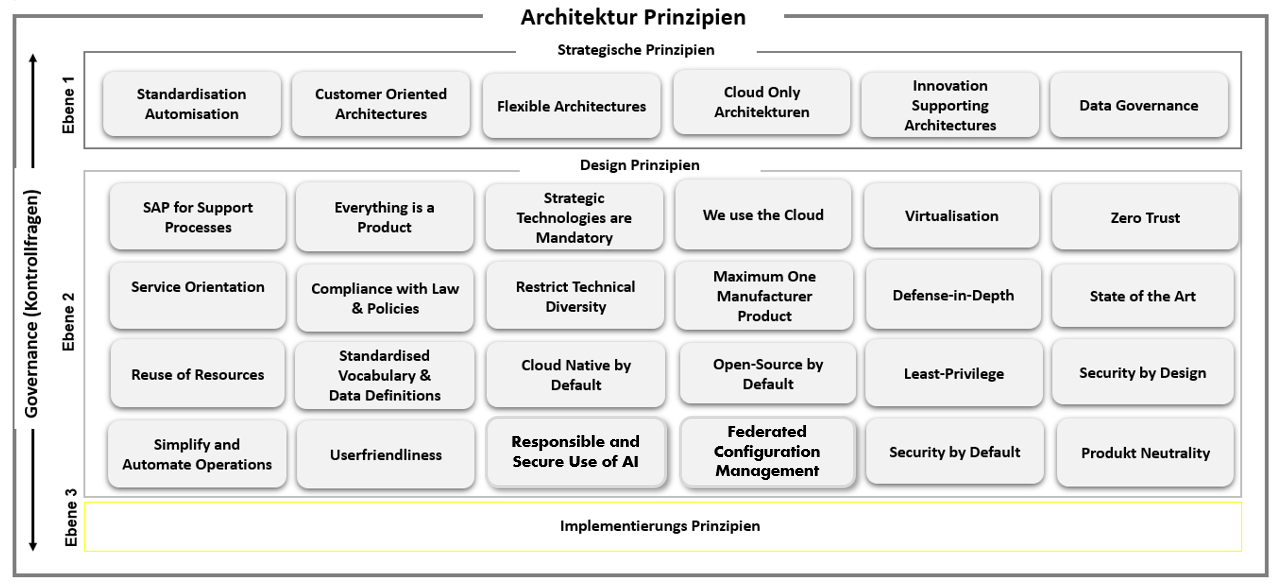
\includegraphics[width=\textwidth]{graphics/bit-architektur-prinzipien.png}
    \caption{Architekturprinzipien des \ac{bit} \parencite{noauthor_vorgabenportal_2025}}
    \label{fig:bit-architecture-principles}
\end{figure}

Für diese Arbeit werden die Prinzipien je nach gewähltem Use-Case selektiv berücksichtigt. Zu den Kriterien des \ac{bit} sollen weitere identifiziert werden, welche explizit für den Umstand der multi-Cloud ready \ac{ea} vorgesehen sind. Hierfür werden initial die folgenden Recherchefragen formuliert:

\flqq What are possible architecture princples for multi-Cloud ready enterprise architectures and solution architectures?\frqq\hspace{0.05cm}, welche mit Elicit AI recherchiert wurde (siehe Tools in \fullref{sec:hilfsmittel}). Die identifizierten Prinzipien zeigen, dass die Frage mit dem Begriff \flqq solution architecture\frqq\hspace{0.05cm} bereits zu stark auf konkrete technische Prinzipien fokussiert, siehe \fullref{appendix:architecture-principles-v1}. Dies entspricht nicht dem angedachten Abstraktionsniveau für Prinzipien einer \ac{ea}, weshalb die adaptierte Recherchefrage wie folgt lautet: \flqq Which normative, technology-agnostic enterprise architecture principles must hold so that multiple cloud-specific solution architectures can be derived consistently?\frqq. Die identifizierten Architekturprinzipien in \autoref{tab:architecture-principles} entstanden unter anderem basierend auf dem Screening von Abstracts nach Enterprise Architecture Priniples und dem Bezug von Cloud Computing Architecture bzw. multi-Cloud Environments siehe \fullref{appendix:architecture-principles-v2}.

\begin{longtable}{|
  L{3cm}|
  p{\dimexpr\textwidth-6cm-6\tabcolsep-4\arrayrulewidth\relax}|
  L{3cm}|
}
    \hline
    \textbf{Prinzip} & \textbf{Beschreibung} & \textbf{Quellen} \\
    \hline
    \endfirsthead

    \hline
    \textbf{Prinzip} & \textbf{Beschreibung} & \textbf{Quellen} \\
    \hline
    \endhead

    Architectural Abtraction Principle &
    Architektur soll mittels Abstraktion businessspezifische Elemente von cloudspezifischen Implementationen loslösen. Durch konkrete technologische Elemente wie Containerisierung und plattform-agnostische Interfaces kann somit eine Portabilität erreicht werden &
    \cite{srikanth_gurram_multi-cloud_2025}, \cite{erl_cloud_2013}
    \\
    \hline
    Modular Decomposition Prinicple &
    Architektur soll Zerlegung von Cloud-Stacks in Komponenten gewährleisten. Dies soll eine Nutzung von Funktionen über Cloud-Tiers hinweg ermöglichen und eine starre Bindung an einen Anbieter verhindern &
    \cite{papazoglou_cloud_2012}, \cite{tritsiniotis_get_2016}
    \\
    \hline
    Reference Model Principle &
    Architektur soll auf Referenzmodellen aufbauen. Diese Modelle bilden eine gemeinsame Sprache für die architektonische Integrität und dienen als Leitfaden für die Identifizierung, Klassifizierung und Einführung von Technologien &
    \cite{kratzke_clouns_2016}, \cite{zhang_ccoa_2009}
    \\
    \hline
    Governance Primacy Principle &
    Architektur soll klar auf Policies, Regulations und Unternehmensvorgaben aufbauen und nicht durch Technologie motiviert sein. Dies erreicht, dass trotz Unterschieden in den konkreten Lösungen / Cloud-Plattformen die Governancen als Input für das Vorgehen im Vordergrund bleibt &
    \cite{zhang_ccoa_2009}, \cite{gurram_multi-cloud_2025}
    \\
    \hline
    Security Reconfigurability Principle &
    Security Architektur soll auf einer allgemeingültigen Security-Absicht aufbauen. Dieses dient wiederum als Ausgangslage für konkrete Security Models und deren spezifische Umsetzung pro Cloud-Plattformen. Absichten und Models, welche bereits zu stark auf eine Plattform fokussieren, stellen das Risiko dar, dass sie nicht auf einer anderen Cloud-Plattform anwendbar sind &
    \cite{hajjat_cloudward_2010}
    \\
    \hline
    \caption{Potenzielle Architekturprinzipien für eine multi-Cloud enabled \ac{ea} siehe \autoref{appendix:architecture-principles-v2} }
    \label{tab:architecture-principles}
\end{longtable}

Für die Qualitätsmerkmale werden sowohl eigens definierte Kriterien als auch jene aus der Recherche verwendet. Hierfür wird folgende Fragestellung verwendet: \flqq Which architecture-related quality attributes are suitable for the comparative evaluation of enterprise architectures in technology-agnostic multi-Cloud environments?\frqq. Das Ergebnis gliedert sich in die folgenden Tiers: Tier 1 Universable Applicable, Tier 2 Context-Dependent Critical, Tier 3 Multi-cloud Specific, Tier 4 Emerging Considerations. Von Interesse sind hierbei vor allem die Kriterien, welche sich explizit auf den multi-Cloud Aspekt beziehen, sprich dem Tier 3.

\begin{longtable}{|L{1cm}|L{3cm}|p{\dimexpr\textwidth-8cm-6\tabcolsep-4\arrayrulewidth}|L{4cm}|}
    \hline

    \textbf{Tier} & \textbf{Quality Attribute} & \textbf{Beschreibung im \ac{ea} Kontext} & \textbf{Quellen} \\
    \hline
    \endfirsthead

    \hline
    \textbf{Tier} & \textbf{Quality Attribute} & \textbf{Beschreibung im \ac{ea} Kontext} & \textbf{Quellen} \\
    \hline
    \endhead

    1 &
    Performance &
    Fähigkeit gewisse Antwortzeiten und Durchsatzraten zu gewährleisten sowie Fähigkeit auf Workload-Anpassungen zu reagieren &
    \cite{papaioannou_architecture_2013}, \cite{bhargav_sai_pillati_leading_2025}, \cite{banijamali_software_2019}, \cite{mohammad_asad_hussain_comparative_2025}
    \\
    \hline
    1 &
    Reliability &
    Fähigkeit ein beständiges Sericeverhalten zu haben sowie Service Level Objectives einzuhalten. Fokus liegt auf der allgemeinen Robustheit, statt nur Ausfallsicherheit zu gewährleisten &
    \cite{papaioannou_architecture_2013}, \cite{bhargav_sai_pillati_leading_2025}, \cite{banijamali_software_2019}
    \\
    \hline
    1 &
    Cost-effectiveness &
    Fähigkeit Kosten transparent abzubilden um eine Vergleichbarkeit zu ermöglichen sowie Fähigkeit Möglichkeit zur Optimierung der Kosten zu geben - nicht nur zwangsläufig tiefstmögliche Kosten &
    \cite{papaioannou_architecture_2013}, \cite{bhargav_sai_pillati_leading_2025}, \cite{menzel_cloudgenius_2011}
    \\
    \hline
    2 &
    Security &
    Fähigkeit Security-Ziele konsistent enforcen zu können sowie Fähigkeit Governancen und Policy-Enforcement zu ermöglichen &
    \cite{bhargav_sai_pillati_leading_2025}, \cite{banijamali_software_2019}, \cite{ghazaryan_comparative_2025}
    \\
    \hline
    2 &
    Scalability &
    Fähigkeit mit Anpassungen in der Workload-, Daten, Nutzergrösse etc. umzugehen ohne strukturelle Änderungen vornehmen zu müssen &
    \cite{bhargav_sai_pillati_leading_2025}, \cite{banijamali_software_2019}, \cite{mohammad_asad_hussain_comparative_2025}
    \\
    \hline
    2 &
    Availability &
    Fähigkeit eine gewisse Verfügbarkeit zu gewährleisten sowie Fähigkeit Redundanz-Strategien sowie High-Availability zu unterstützen &
    \cite{banijamali_software_2019}, \cite{ardagna_modaclouds_2012}
    \\
    \hline
    3 &
    Interoperability &
    Fähigkeit Interaktion und Integration zwischen Systemen auf unterschiedlichen Plattformen zu erlauben &
    \cite{banijamali_software_2019}, \cite{joukov_cloud_2013}
    \\
    \hline
    3 &
    Portability &
    Fähigkeit der Architektur eine Migration oder Redeployment zwischen verschiedenen Plattformen zu erlauben, ohne grundsätzliches Redesign zu benötigen - bspw. ermöglicht durch Abstraktion &
    \cite{mirsalari_model_2020}
    \\
    \hline
    3 &
    Vendor-Neutrality &
    Fähigkeit der Architektur strukturell von einem Anbieter und insbesondere von proprietären Funktionen abhängig zu sein. &
    \cite{bhargav_sai_pillati_leading_2025}
    \\
    \hline
    4 &
    Service Adaptability &
    Fähigkeit der Architektur Änderungen von Anforderungen, Interfaces oder dem Integrations-Kontext unterzubringen ohne die Architektur fundamental zu verändern. Service sind hierbei im Sinne der Capability zu verstehen, nicht ein konkreter technische Service Implementation &
    \cite{bhargav_sai_pillati_leading_2025}
    \\
    \hline
    4 &
    Architectural Sustainability &
    Fähigkeit der Architektur sich langfristig an ändernde technologische sowie organisatorische Gegebenheiten anpassen zu können. Die Differenzierung zur Portability und Interoperability ist, dass diese auch längerfristig aufrechterhalten werden können &
    \cite{bhargav_sai_pillati_leading_2025}
    \\
    \hline
    \caption{Quality-Attriute aus Recherche nach \autoref{appendix:quality-attributes-research} }
    \label{tab:quality-attributes-external}
\end{longtable}

Zu den externen Quality-Attributes kommen eigene Kriterien hinzu welche basierend auf der Traceability-Architecture definiert werden.

\begin{longtable}{|
  L{3cm}|
  p{\dimexpr(\textwidth-3cm-6\tabcolsep-4\arrayrulewidth)/2}|
  p{\dimexpr(\textwidth-3cm-6\tabcolsep-4\arrayrulewidth)/2}|
}
    \hline

    \textbf{Quality Attribute} & \textbf{Beschreibung im Kontext der Traceability-Architecture} & \textbf{Begründung} \\
    \hline
    \endfirsthead

    \hline
    \textbf{Quality Attribute} & \textbf{Beschreibung im Kontext der Traceability-Architecture} & \textbf{Begründung} \\
    \hline
    \endhead

    Auditability &
    Fähigkeit die beschreibt wie nachvollziehbar die Zuweisung von Control und Assignment sind. Dies beinhaltet ebenfalls die verantwortlichen Akteure und Entscheidungspfade welche zum Assignment geführt haben. &
    Für die Generierung von Evidence für Governance und Compliance ist eine Auditierbarkeit essenziell
    \\
    \hline

    Automatability &
    Fähigkeit, dass Traceability-Beziehungen, Prüfungen und Nachweise automatisch erzeugt werden können. Dies beinhaltet ebenfalls die Zuweisung der Controls &
    Automatisierung soll den manuellen Aufwand und die Fehleranfälligkeit der Architektur reduzieren. Bei hoher Komplexität und Anzahl Artefakte gewinnt dies umso mehr Relevanz
    \\
    \hline

    Maintainability &
    Aufwand die Traceability-Modelle, Beziehungen und Controls aktuell zu halten &
    Policies auf den Plattformen und damit Zuweisungen zu entsprechenden Controls ändern sich regelmässig.
    \\
    \hline

    Adaptability &
    Fähigkeit in der Architektur neue Traceability-Beziehungen, Artefakt-Typen, Controls etc. hinzuzufügen ohne die Architektur grundlegend überarbeiten zu müssen &
    Cloud-Plattformen sowie relevante Regulatorien können sich ändern.
    \\
    \hline

    Multi-Cloud Applicability &
    Grad der Fähigkeit in der die Architektur über verschiedene Cloud-Plattormen konsistent anwendbar ist, ohne das strukturelle Änderungen notwendig sind. &
    Es wird bereits vorausgesetzt, dass eine grundsätzliche Multi-Cloud Fähigkeit besteht. Mit diesem Kriterium wird eine Vergleichbarkeit erreicht.
    \\
    \hline

    Complexity &
    Grad der zusätzlichen Vielschichtigkeit und Tiefe der Architektur. Es ist nicht die grundsätzlich Komplexität einer Architektur gemeint, sondern ein etwaiges Übermass an Komplexität in Anbetracht des Problems welches gelöst werden soll &
    Bei der Traceability handelt es sich bereits von Natur aus um eine vielschichtige Thematik. Entsprechend sollte vermieden werden das durch zu hohe Abstraktionen die Komplexität unverhältnismässig ist.
    \\
    \hline

    Traceability Strength &
    Grad in der die Beziehung zwischen Anwendung auf einer Cloud-Ressource zu der ausgehen Control hergestellt werden kann &
    Es wird bereits vorausgesetzt, dass eine grundsätzliche Traceability besteht. Mit diesem Kriterium wird eine Vergleichbarkeit erreicht.
    \\
    \hline

    \caption{Dedizierte Quality-Attriute mit Fokus auf Traceability-Architecture}
    \label{tab:quality-attributes}
\end{longtable}

Für die Dimension der Trade-Off Kriterien wird für die Recherche von Spannungsfeldern folgende Fragestellung verwendet: \flqq Which architecture-level trade-offs shape the design and evaluation of enterprise architectures in technology-agnostic multi-Cloud environments\frqq.

\begin{longtable}{|
  L{3cm}|
  p{\dimexpr\textwidth-6cm-6\tabcolsep-4\arrayrulewidth\relax}|
  L{3cm}|
}
    \hline
    \textbf{Trade-Off Dimension} & \textbf{Spannungsfeld} & \textbf{Quellen} \\
    \hline
    \endfirsthead

    \hline
    \textbf{Trade-Off Dimension} & \textbf{Spannungsfeld} & \textbf{Quellen} \\
    \hline
    \endhead

    Performance vs Portability &
    Optimieren der Runtime-Effizienz steht in Konflikt mit der langfristigen architektonischen Mobilität, da die Runtime-Effizienz häufig durch Optimierung auf ein bestimmtes Umfeld erreicht wird.

    Tendenz zu Performance führt zur bestmöglichen Ausnutzung von cloud-nativen Capabilities und tiefen Latenzen aber dafür verliert man an architektonischer Unabhängigkeit vom Provider und Vergleichbarkeit von Lösungen über Cloud-Plattformen hinweg. &
    \cite{gibilisco_methodology_2016}, \cite{emmanni_architecting_2020}, \cite{papaioannou_architecture_2013-1}
    \\
    \hline

    Cost effectiveness vs Architectural specialization &
    Transparente Abbildung der Kosten sorgt für die Möglichkeit der Zuweisbarkeit von Kosten zu Architekturelementen. Dies erlaubt eine Vergleichbarkeit und das Senken des Risikos unerwarteter Kosten. Architecture specialization ermöglicht es wiederum  spezialisierte / stark integrierte Services einzusetzen, welche die Kostenmodelle jedoch verkomplizieren. Eine Architektur die Kosten transparent hält, vermeidet tendenziell stark gekoppelte oder schwer kalkulierbare Strukturen &
    \cite{arul_data_2022}, \cite{sai_leading_2025}, \cite{emmanni_architecting_2020}
    \\
    \hline

    Flexibility vs Structural simplicity &
    Flexibilität sorgt dafür, dass auf neue Requirements eingegangen werden kann und entsprechend eine bessere Anpassungsfähigkeit besteht. Gleichzeitig sinkt mit der steigenden Anzahl an architektonischen Konzepten und Optionen die Einfachheit der Architektur. Durch die Structural simplcity gibt es weniger Konzepte welche dafür klar definiert sind was zu einer besseren Verständlichkeit führt. Änderungen an Requirements manifestieren sich somit aber auch mehr in strukturellen Änderungen.
    
    Die genannten Quellen fokussieren vor allem auf Flexibility vs Complexity. Da Complexity jedoch in \autoref{tab:quality-attributes} jedoch als zusätzlicher Abstraktion beschrieben wurde, wurde hier Structural simplicity als Dimension gewählt&
    \cite{gibilisco_methodology_2016}, \cite{papaioannou_architecture_2013}, \cite{arul_data_2022}
    \\
    \hline

    Security vs Usability &
    Security führt zu mehr Sicherheitsmechanismen, welche den Schutzgrad erhöhen sollen aber auch gleichzeitig zu operativen höheren Hürden führt. Mit der Usability wird die Architektur hingegen einfacher nutzbar und integrierbar. Es vereinfacht sich jedoch auch das Sicherheitsmodell bzw. Kontrollinstanzen
    &
    \cite{berlato_exploring_2020}, \cite{casola_security-by-design_2018}
    \\
    \hline

    Vendor Lock-In vs Scalability &
    Scalability bzw. provider-native Optimierung führt zur Steigerung der Effizienz und Nutzung von Plattformspezifischer Skalierung, Verwaltung etc. Gleichzeitig erhöht sich jedoch die Abhängigkeit von bestimmten Anbieter. Vendor Lock-In Vermeidung hingegen bringt provider-neutrale Architekturen mit sich, welche die strategische Unabhängigkeit steigern. Mit dieser Steigerung der Austauschbarkeit sinkt jedoch die Nutzung von Provider-spezifischen Funktionen
    &
    \cite{berlato_exploring_2020}, \cite{quint_towards_2018}, \cite{zhao_supporting_2022}
    \\
    \hline

    \caption{Trade-Off Dimensionen aus der Recherche in \autoref{appendix:trade-off-criteria-reserach}}
    \label{tab:tension-fields-external}
\end{longtable}

Zusätzlich zu den Trade-Off Dimensionen aus der Literatur werden die folgenden spezifischen Dimensionen definiert welche die Limitationen aus gewissen Architekturprinzipien bereits berücksichtigen und welche sich explizit auf die Traceability-Architecture beziehen.

\begin{longtable}{|
  L{3cm}|
  p{\dimexpr\textwidth-6cm-6\tabcolsep-4\arrayrulewidth\relax}|
  L{3cm}|
}
    \hline
    \textbf{Trade-Off Dimension} & \textbf{Spannungsfeld} & \textbf{Begründung} \\
    \hline
    \endfirsthead

    \hline
    \textbf{Trade-Off Dimension} & \textbf{Spannungsfeld} & \textbf{Begründung} \\
    \hline
    \endhead
    
    Traceability Depth vs. Model Simplicity &
    Mit einer tiefen Traceability Depth werden mehr Artefakte modelliert und tiefere Traceability-Ketten generiert, womit Zusammenhänge besser rekonstruiert werden können. Die Model Simplicity führt dazu, dass das Metamodell überschaubarer bleibt, jedoch auch zu Verlust von Detailinformationen &
    Relevant basierend auf den Anforderungen was für Evidenz / Artefakte erstellt werden möchte
    \\
    \hline

    Explicit Trace Modeling vs. Implicit Derivation &
    Mit explicit Tracing werden Beziehungen zwischen den Objekten im Metamodell bewusst modelliert, womit auch der initiale Modellierungsaufwand steigt. Dies führt zu einer besseren Prüfbarkeit und Auditierarkeit. Die implicit Derivation leitet Traceability-Beziehungen aus ggf. bestehenden Regeln oder Strukturen ab, womit die Abhängigkeit von implizitem Wissen steigt. &
    Relevant wegen der Abhängigkeit die sich aus der Abhängigkeit zu Modellierung von Cloud-Providern aber auch dem Aufwand die sich aus einer eigenen Modellierung ergibt
    \\
    \hline

    Central Traceability Model vs. Federated Traceability Models &
    Mit dem central Model wird ein einheitliches Model mit semantischer Vergleichbarkeit angestrebt, was eine einfachere domänenübergreifende Auswertung erlaubt. Mit dem federated Model existiert eine gewisse Vielfalt für eine Domäne, welche durch eine Auswertung zentral gemapped werden muss. Die Konsistenz entsteht durch eine zentrale Auswertung / Mapping &
    Relevant je nach Heterogenität der Domänen, um keine künstlichen Modelle zu erhalten die ggf. domänenspezifische Strukturen einschränken
    \\
    \hline

    Governance centric Traceability vs. Engineering centric Traceability &
    Eine governance-centric Traceability setzt die Policies, Controls und Compliance in den Fokus. Die Traceability ist hierbei top-down angedacht. Der Fokus liegt hierbei hauptsächlich auf der Auditierbarkeit, was dem Fokus bspw. eines Compliance Officers entspricht. Die engineering-centric Traceability bringt die technische Nachvollziehbarkeit und die technische Implementierungen / Artefakte in den Fokus. Dies entspricht potenziell der Betrachtung eines Entwicklers &
    Relevant für die Wahl der Betrachtungsrichtung welche gewählt wird.
    \\
    \hline

    Static Traceability Structure vs. Evolvable Traceability Structure &
    Eine static Structure ist bewusst in stabilen Strukturen angedacht, bei der Änderungen nicht häufig passieren sollen. Dadurch wird auch langfristig eine Vergleichbarkeit erreicht. Die evolvable Structure bezieht sich auf die bewusste Anpassung und Erweiterung von Artefakt-Typen. Es wird somit bewusst offen definiert, um erweiterbar zu sein, was jedoch eine Vergleichbarkeit über die Zeit erschwert &
    Relevant für die Vergleichbarkeit von auf der Architektur generierten Artefakten wie Audits
    \\
    \hline

    High Formalization vs. Interpretative Flexibility &
    In einer Architektur mit high Formalization sind die Traceability-Konzepte oder Regeln klar definiert und maschinenlesbar. Hierdurch wird eine Automatisierbarkeit und Vergleichbarkeit erreicht, verliert jedoch man pragmatische Anpassungen an Domänen mit unscharfer Semantik oder Informationen. In einer Architektur mit interpretive Flexibility können Traceability Beziehungen nicht vollständig formalisiert sein und semantische Lücken bewusst toleriert werden. Die Interpretation erfolgt manuell oder teil-automatisiert durch Menschen mit Kontextwissen &
    Relevant basierend auf dem Prozess der angestrebt wird. Soll der Mensch aktiv in the loop sein oder wird eine volle Automatisierung angestrebt
    \\
    \hline

    Traceability Coverage vs. Traceability Precision &
    Bei Architekturen mit hoher Traceability Coverage zielen darauf ab, möglichst viele Artefakte, Beziehungen und Prozesse abzubilden. Dies führt zu hoher Transparenz und Vollständigkeit. Jedoch kann hierbei auch Overhead oder ein Rauschen entstehen welches die Interpretation erschwert. Bei Traceability Precision wird Wert darauf gelegt, die Beziehungen so präzise wie möglich darzustellen, um eine bessere Aussagekraft, klarere Prüfbarkeit und bessere Nachvollziehbarkeit zu erreichen. &
    Relevant für das Setzen des Fokus auf breite oder tiefe der Traceability je nach Anwendungsfall (z.B. Audit vs. Incident Investigation)
    \\
    \hline

    Policy-driven Traceability vs. Control-driven Traceability &
    Bei der Policy-driven Traceability wird von den Richtlinien, Standards und Governance-Vorgaben aus gearbeitet: \textit{was} muss nachgewiesen werden? Dies führt zu einheitlicher Auditierbarkeit jedoch potenziell auch zu Überdokumentation und fehlender technischer Relevanz. Bei Control-driven wird von den verfügbaren Controls aus die Auditierbarkeit einer Anwendung aufgebaut. Dies bringt hohe technische Relevanz und im Engineering verankerte Auditierbarkeit aber auch die Gefahr mit sich, nicht alle übergeordneten Regulatorien abzudecken. Eine Kombination der beiden Ansätze wäre möglich, muss jedoch im Voraus festgelegt werden. &
    Relevant für die Entscheidung von welcher Sicht aus die Traceability aufgebaut werden soll
    \\
    \hline
    \caption{Selbst definierte Trade-Off Dimensionen}
    \label{tab:tension-fields}
\end{longtable}

Die Dimension des Kontextes und der Anwendung wie beschrieben in \autoref{tab:evaluation-dimensions} stellt keine eigentliche Bewertungsdimension, sondern eine Gewichtungsdimension dar. Dies bedeutet, dass diese Dimensionen keinen Anspruch auf Objektivität erheben und sich nicht zwangsläufig mit bestehender Literatur decken. In dieser Arbeit werden als Kontext die definierten Use-Cases für das \ac{bit} in \autoref{sec:methodik-capability} verwendet.

\subsubsection{Konformitätsprozess für die Traceability-Architektur}
\label{sec:conformityprocess-architecture}

Mittels der Dimension \flqq Architekturprinzipien\frqq\ wird ein Konformitätsprozess definiert. Der Prozess wendet die verschiedenen Prinzipien auf die Traceability-Architektur an um eine Aussage über die Konformität machen zu können. Diese Aussage soll aufzeigen, dass die Struktur der Traceability-Architektur den Anforderungen aus der Dimension \flqq Kontext und Anwendung\frqq\ entspricht.

\hl{Evaluierung hier ist nicht mehr aktuell, da die prinzipien nur noch als fail pass beurteilt wreden}

\begin{align}
P &= \{p_1, \dots, p_n\}  \\
P_{\text{selection}} &= \{\, p \in P \mid p \text{ ist Teil der Auswahl } \,\} \\ \\
\end{align}

Zur Fokussierung auf den Kontext, in welchem die Konformität gezeigt werden soll, wird eine Ausahl der Architekturprinzipien aus \autoref{fig:bit-architecture-principles} und \autoref{tab:architecture-principles} vorgenommen. Diese Auswahl wird als $P_{\text{selection}}$ bezeichnet.

\begin{align}
s_{\text{principles}} &: P \rightarrow \{0, 1, 2, 3, 4\}
\end{align}

Das Mass der Erfüllung eines Architekturprinzips wird mit $s_{\text{principles}}(p)$ ermittelt.

\begin{align}
s_{\text{principles}}(p) =
\begin{cases}
< 1, & \text{falls Prinzip } p \text{ Prinzip nicht erfüllt } \\
>= 1 & \text{falls Prinzip } p \text{ Prinzip erfüllt }
\end{cases}
\end{align}

Ein Architekturprinzip, welches mit $w_{\text{principles}}(p) = 0$ resultiert, gilt als nicht erfüllt und bedeutet, dass die Architektur den Konformitätschecks nicht bestanden hat.

\begin{align}
passed = \forall p \in P_{\text{selection}} \; ( s_{\text{principles}}(p) > 0 )
\end{align}

Damit der Konformitätschecks als erfüllt gilt, müssen alle Architekturprinzipien in einem Mindestmass mit $passed$ erfüllt werden.

\begin{longtable}{|
  L{1cm}|
  p{\dimexpr\textwidth-4cm-6\tabcolsep-4\arrayrulewidth\relax}|
  L{3cm}|
}
    \hline
    \textbf{Nr} & \textbf{Beschreibung} & \textbf{Output} \\
    \hline
    \endfirsthead

    \hline
    \textbf{Nr} & \textbf{Beschreibung} & \textbf{Output} \\
    \hline
    \endhead

    \hline
    \multicolumn{3}{|c|}{\textbf{Initialisierung}} \\
    \hline

    1 & Definieren vom Kontext und darauf aufbauend Leitgedanken, mit welchen die Bestimmung von Parametern hergeleitet werden kann. Diese können bspw. auf Use-Cases aufbauen &
    Beschreibung des Kontextes
    \\
    \hline

    2 & Auswahl der Architekturprinzipien vornehmen aus \autoref{fig:bit-architecture-principles} und \autoref{tab:architecture-principles}  &
    Liste der Auswahl an Architekturprinzipien $P_{\text{selection}}$
    \\
    \hline

    \multicolumn{3}{|c|}{\textbf{Anwendung auf Traceability-Architektur}} \\
    \hline

    3 & Bewerten der Traceability-Architektur basierend auf allen Architekturprinzipien in $P_{\text{selection}}$ mit den Punkten aus  $s_{\text{principles}}$  &
    Bewertung $s_{\text{principles}}(p)$
    \\
    \hline

    4 & Verfassen einer Gesamtbewertung basierend auf den vorherigen Ergebnissen & Gesamtbewertung der Variante
    \\
    \hline

    \caption{Konformitätscheck mit den einzelnen nummerierten Schritten}
    \label{tab:archicture-conformity-process}
\end{longtable}

Für die Anwendung des Konformitätsprozess wird in der Initialisierung nachfolgende Auswahl $P_{\text{selection}}$ vorgenommen. Diese werden in folgende Gruppen eingeordnet um bei der Beurteilung der Konformität verschiedene Themen kombinieren zu können:

\begin{itemize}
  \item Gruppe 1: Governance-Driven Architecture
  \item Gruppe 2: Abstraction and Plattform Independence
  \item Gruppe 3: Structural Architecture
  \item Gruppe 4: Security Architecture
\end{itemize}
\label{tab:selection-architecture-principles}

\paragraph{Gruppe 1: Governance-Driven Architecture}

\textbf{A1}: \textbf{Compliance with Law and Policies} \hypertarget{architecture-a1}{}

Wir beim BIT stellen sicher, dass wir die Gesetze, Vorschriften und Richtlinien einhalten, einschliesslich der Bundes-, Departements- und Amts-Prinzipien.
\textbf{Begründung}: Die Nachvollziehbarkeit und das Enforcement von Regulationen ist einer der Beweggründe im Use-Case für die Traceability.
\textbf{Quelle}: Auszug aus \autoref{fig:bit-architecture-principles}

\textbf{A2}: \textbf{Data Governance} \hypertarget{architecture-a2}{}

Wir stellen sicher, dass wir als Leistungsbezüger \ac{bit}-Daten mit klar definierten Regeln, Richtlinien und Praktiken verwalten, die die Qualität, Zugänglichkeit und Konsistenz der Daten gewährleisten. 
\textbf{Begründung}: Für das Placement der Foundation ist die Berücksichtigung der Datenklassifizierung ausschlaggebend.
\textbf{Quelle}: Auszug aus \autoref{fig:bit-architecture-principles}

\paragraph{Gruppe 2: Abstraction and Plattform Independence}

\textbf{A3}: \textbf{Cloud-native by Default} \hypertarget{architecture-a3}{}

Wir entwickeln und betreiben Cloud-native Anwendungen.
\textbf{Begründung}: Der Lösungsansatz welcher durch Traceability-Architektur vorgeschlagen wird soll sich bereits möglichst nah am Umfeld orientieren in welchem es eingesetzt wird.
\textbf{Quelle}: Auszug aus \autoref{fig:bit-architecture-principles}, sowie \cite{srikanth_gurram_multi-cloud_2025}, \cite{erl_cloud_2013}

\textbf{A4}: \textbf{Architectural Abstraction Principle} \hypertarget{architecture-a4}{}

Architektur soll mittels Abstraktion Business-spezifische Elemente von Cloud-spezifischen Implementationen loslösen. Durch konkrete technologische Elemente wie bspw. Containerisierung und Plattform-agnostische Interfaces kann somit eine Portabilität erreicht werden.
\textbf{Begründung}: Um den unterschiedlichen Implementationen der Cloud-Provider gerecht zu werden ist eine Abstraktion für die Traceability unerlässlich.
\textbf{Quelle}: \cite{srikanth_gurram_multi-cloud_2025}, \cite{erl_cloud_2013}

\textbf{A5}: \textbf{Product Neutrality} \hypertarget{architecture-a5}{}

Die Sicherheitsvorgaben im BIT adressieren Anforderungen und keine Herstellerprodukte.
\textbf{Begründung}: Herstellerspezifische Konzepte sollten bereits auf der Ebene der Architektur ausgeschlossen werden und höchstens konzeptionell betrachtet werden.
\textbf{Quelle}: Auszug aus \autoref{fig:bit-architecture-principles}

\paragraph{Gruppe 3: Structural Architecture}

\textbf{A6}: \textbf{Serviceorientation} \hypertarget{architecture-a6}{}

Wir beim BIT stellen sicher, dass unsere Lösungen auf einem Design von Dienstleistungen basieren, welche die realen Geschäftsaktivitäten widerspiegeln und die Geschäftsprozesse des Unternehmens (oder zwischen Unternehmen) umfassen.
\textbf{Begründung}: Die Traceability-Architektur soll sich an den verschiedenen Akteuren aus dem Use-Case ausrichten, um bereits eine optimale Ausrichtung auf potenzielle Anwender zu gewährleisten.
\textbf{Quelle}: Auszug aus \autoref{fig:bit-architecture-principles}

\textbf{A7}: \textbf{Modular Decomposition Principle} \hypertarget{architecture-a7}{}

Architektur soll Zerlegung von Cloud-Stacks in Komponenten gewährleisten. Dies soll eine Nutzung von Funktionen über Cloud-Tiers hinweg ermöglichen und eine starre Bindung an einen Anbieter verhindern.
\textbf{Begründung}: Analog wie die Product Neutrality sollen nicht nur Konzepte, sondern auch die Komponenten der Architektur agnostisch gedacht werden.
\textbf{Quelle}: \cite{papazoglou_cloud_2012}, \cite{tritsiniotis_get_2016}

\textbf{A8}: \textbf{Reference Model Principle}\hypertarget{architecture-a8}{}

Architektur soll auf Referenzmodellen aufbauen. Diese Modelle bilden eine gemeinsame Sprache für die architektonische Integrität und dienen als Leitfaden für die Identifizierung, Klassifizierung und Einführung von Technologien, siehe \autoref{tab:architecture-principles}.
\textbf{Begründung}: Traceability selbst ist bereits ein abstrakter Begriff. Ein Metamodell welche ein Mapping auf Cloud-Plattform spezifische Namen und Konzepte ermöglicht ist deshalb relevant.
\textbf{Quelle}: \cite{kratzke_clouns_2016}, \cite{zhang_ccoa_2009}

\textbf{A9}: \textbf{Standardisation Automation} \hypertarget{architecture-a9}{}

Wir streben danach, alle Bausteine unserer Architekturen so weit wie möglich zu standardisieren und die Prozesse so weit wie möglich zu automatisieren. Dieser Ansatz gilt für Geschäftsprozesse, Datenstrukturen, Daten, Anwendungen, Anwendungskomponenten und Infrastrukturkomponenten.
\textbf{Begründung}: Die Automatisierung der Compliance-Prüfung ist einer der Hauptversprechen der Traceability-Architektur. Der Aufbau einer möglichst standardisierten Struktur für die Abbildung der Traceability und Evidences ist deshalb relevant.
\textbf{Quelle}: Auszug aus \autoref{fig:bit-architecture-principles}

\paragraph{Gruppe 4: Security Architecture}

\textbf{A10}: \textbf{Security by Design} \hypertarget{architecture-a10}{}

Sicherheitsanforderungen an Software sowie Hardware werden bereits in der Entwicklung berücksichtigt, um spätere Schwachstellen in der Sicherheit zu verhindern.
\textbf{Begründung}: Mit der Traceability selbst soll die Durchsetzbarkeit der Regulation wie \ac{si001} erhöht werden. Dies gilt auch für die Konzeption der Traceability-Architekur als solche.
\textbf{Quelle}: Auszug aus \autoref{fig:bit-architecture-principles}

\textbf{A11}: \textbf{Defense-In-Depth} \hypertarget{architecture-a11}{}

Es braucht mehrere komplementäre Massnahmen aus den Bereichen Personal, Technologie und Betrieb um eine Information effektiv zu schützen.
\textbf{Begründung}: Da es sich bei der Traceability-Architektur selbst um ein Werkzeug für Audits der Foundations handelt, sind Sicherheitsüberlegung noch wichtiger.
\textbf{Quelle}: Auszug aus \autoref{fig:bit-architecture-principles}

\textbf{A12}: \textbf{Security Reconfigurability Principle} \hypertarget{architecture-a12}{}

Security soll auf einer allgemeingültigen Security-Absicht aufbauen. Dieses dient wiederum als Ausgangslage für konkrete Security Models und deren spezifische Umsetzung auf den Cloud-Plattformen. Absichten und Models, welche bereits zu stark auf eine Plattform fokussieren stellen das Risiko dar, dass sie nicht auf einer anderen Cloud-Plattform anwendbar sind, siehe \autoref{tab:architecture-principles}.
\textbf{Begründung}: Die Annahmen auf welcher die Traceability-Architektur strukturiert sowie weitere Konzepte erarbeitet werden sollte Plattform-übergreifend anwendbar sein.
\textbf{Quelle}: \cite{hajjat_cloudward_2010}

\subsubsection{Evaluationsprozess für die Varianten der Traceability-Architektur}
\label{sec:evaluationprocess-traceability-variants}

Mittels der Dimensionen \flqq Qualitätsmerkmale\frqq\ und \flqq Entscheidung und Trade-Off\frqq\ wird ein Evaluationsprozess definiert. Der Evaluationsprozess wendet die verschiedenen Dimensionen an um einen bewertenden Output generieren zu können. Durch Anwendung des Prozesses auf die verschiedenen Traceability-Architektur-Varianten soll eine Vergleichbarkeit ermöglicht werden. Schlussendlich kann somit eine Empfehlung im Anwendungskontext gegeben werden. Gedanklich orientiert sich dieser Prozess somit an einer \ac{MCDA} in der verschiedene Konfliktbereiche zueinander ins Verhältnis gesetzt werden.

Der Output des Prozesses ist der $Score_{\text{quality}}$ kombiniert mit einer textuellen Einordnung mittels der Trade-Off Kriterien. Diese Trennung ergibt sich daraus, dass sich die Qualitätsattribute  quantitativ, jedoch die Trade-Off Kriterien nur qualitativ bewerten lassen. Mit dieser Trennung soll die Verständlichkeit der Bewertung erhöht werden. Des Weiteren soll betont werden, dass die Trade-Off Kriterien zur Einordnung des  $Score_{\text{quality}}$ dienen. Als Score wird generell eine bewertende Grösse verstanden.

\begin{align}
Q &= \{q_1, \dots,q_n\} \\
Q_{\text{selection}} &= \{\, q \in Q \mid q \text{ ist Teil der Auswahl } \,\} \\ \\
T &= \{t_1, \dots,t_n\} \\
T_{\text{selection}} &= \{\, t \in T \mid t \text{ ist Teil der Auswahl } \,\} \\ \\
Score_{\text{quality}} &= \frac{\sum_{q \in Q_{\text{selection}}} w_{\text{quality}}(q)\,s_{\text{quality}}(q)} {\sum_{q \in Q_{\text{selection}}} w_{\text{quality}}(q)} \\
\end{align}

Der $Score_{quality}$ ergibt sich aus einer Auswahl an den Qualitätsattributen $Q$ (siehe \autoref{tab:quality-attributes-external} und \autoref{tab:quality-attributes}), welche als $Q_{\text{selection}}$ bezeichnet wird. Die Anzahl an Qualitätsattributen ist durch $|Q_{\text{selection}}|$ gegeben. Zur Gewichtung der einzelnen Merkmale wird $w_{\text{quality}}(p)$ verwendet.

\begin{align}
w_{\text{quality}} &: Q \rightarrow \{0.1, 0.3, 0.4, 0.4, 0.6, 0.7, 0.8, 0.9, 1.0\} \\
s_{\text{quality}} &: Q \rightarrow \{1, 2, 3, 4\}
\end{align}

Die Bewertung des $Score_{\text{quality}}$ erfolgt basierend auf einer Auswahl der Trade-Off Kriterien $T$ (siehe \autoref{tab:tension-fields-external} und \autoref{tab:tension-fields}), welche als $T_{\text{selection}}$ bezeichnet wird.

Mit den beschriebenen Elementen wird folgender Evaluationsprozess definiert:

\begin{longtable}{|
  L{1cm}|
  p{\dimexpr\textwidth-4cm-6\tabcolsep-4\arrayrulewidth\relax}|
  L{3cm}|
}
    \hline
    \textbf{Nr} & \textbf{Beschreibung} & \textbf{Output} \\
    \hline
    \endfirsthead

    \hline
    \textbf{Nr} & \textbf{Beschreibung} & \textbf{Output} \\
    \hline
    \endhead

    \hline
    \multicolumn{3}{|c|}{\textbf{Initialisierung}} \\
    \hline

    1 & Definieren vom Kontext und darauf aufbauend Leitgedanken, mit welchen die Bestimmung von Parametern hergeleitet werden kann. Dies können bspw. auf Use-Cases aufbauen &
    Beschreibung des Kontextes
    \\
    \hline

    2 & Auswahl der Qualitätsattribute vornehmen aus \autoref{tab:quality-attributes-external} und \autoref{tab:quality-attributes}. Anschliessend jedem Qualitätsattribut ein Gewicht $v_i$ entsprechend dem Definitionsbereich zuweisen &
    Liste der Auswahl an Qualitätsattributen mit $Q_{\text{selection}}$ mit Gewichten $w_{\text{quality}}(q)$
    \\
    \hline

    3 & Auswahl der Trade-Off Kriterien vornehmen aus \autoref{tab:tension-fields-external} und \autoref{tab:tension-fields}. Diese werden nicht gewichtet. &
    Liste der Auswahl an Trade-Off Kriterien mit  $T_{\text{selection}}$
    \\
    \hline

    \multicolumn{3}{|c|}{\textbf{Anwendung auf Traceability-Architektur-Variante}} \\
    \hline

    4 & Bewerten Variante basierend auf aller Qualitätsattribute in $Q_{\text{selection}}$ mit den Punkten aus  $s_{\text{quality}}$  &
    Bewertung $s_{\text{quality}}(q)$
    \\
    \hline

    5 & Berechnen des $Score_{\text{quality}}$ &
    Berechneter Score $Score_{\text{quality}}$
    \\
    \hline

    6 & Bewerten der Variante basierend auf den Trade-Off Kriterien $T_{\text{selection}}$ mittels Punkten aus $s_{\text{tradeoff}}$&
    Bewertung $s_{\text{quality}}(q)$ mit der textuellen Begründung
    \\
    \hline

    7 & Verfassen einer Gesamtbewertung basierend auf den vorherigen Ergebnissen & Gesamtbewertung der Variante
    \\
    \hline

    \caption{Evaluationsprozess mit den einzelnen nummerierten Schritten}
    \label{tab:evaluation-process-steps}
\end{longtable}


Für die Anwendung des Evaluationsprozesses wird in der Initialisierung folgende Auswahl für die Qualitätsattribute $Q_{\text{selection}}$ mit den Gewichten $w_{\text{quality}}(q)$ getreoffen.

\begin{longtable}{|
  L{1cm}|
  L{1cm}|
  p{\dimexpr(\textwidth-5cm-10\tabcolsep-6\arrayrulewidth)/2\relax}|
  p{\dimexpr(\textwidth-5cm-10\tabcolsep-6\arrayrulewidth)/2\relax}|
  L{3cm}|
}
    \hline
    \textbf{ID} & \textbf{$w(q)$} & \textbf{Qualitätsattribut} & \textbf{Begründung} & \textbf{Quelle} \\
    \hline
    \endfirsthead

    \hline
    \textbf{ID} & \textbf{$w(q)$} & \textbf{Qualitätsattribut} & \textbf{Begründung} & \textbf{Quelle} \\
    \hline
    \endhead

    Q1 & 0.3 & \textbf{Performance} \hypertarget{quality-q1}{} Fähigkeit gewisse Antwortzeiten und Durchgangsraten zu gewährleisten sowie Fähigkeit auf Workload-Anpassungen zu reagieren & 
    Die Performance ist weniger relevant, da die APIs und Service der Cloud-Provider selbst eine gewisse Durchlaufzeit für die verschiedenen Aktionen haben. Beispiel sind hierbei die Zeitdauer von der Anwendung einer Policy bis zum Erhalt des ersten Resultats  & \cite{papaioannou_architecture_2013}, \cite{bhargav_sai_pillati_leading_2025}, \cite{banijamali_software_2019}, \cite{mohammad_asad_hussain_comparative_2025}
    \\
    \hline

    Q2 & 1 & \textbf{Portability} \hypertarget{quality-q2}{} Fähigkeit der Architektur eine Migration oder Redeployment zwischen verschiedenen Plattformen zu erlauben, ohne grundsätzliches Redesign zu benötigen - bspw. ermöglicht durch Abstraktion &
    Sehr relevant, da die Cloud-Plattformen im \ac{uc} des BIT noch nicht feststehen. Die betrachteten Plattformen Azure und AWS werden lediglich als Beispieke verwedet. Eine Anwendbarkeit auf weitere Cloud-Plattformen ist jedoch essenziell & \cite{mirsalari_model_2020}
    \\
    \hline

    Q3 & 0.6 & \textbf{Auditability} \hypertarget{quality-q3}{} Fähigkeit die beschreibt wie nachvollziehbar die Zuweisung von Control und Assignment sind. Dies beinhaltet ebenfalls die verantwortlichen Akteure und Entscheidungspfade welche zum Assignment geführt haben &
    Die Nachvollziehbarkeit ist relevant, jedoch hauptsächlich für die Traceability selbst und weniger, wann die Beziehungen geändert / angepasst wurden. Die Gewichtung ist deshalb tiefer & \autoref{tab:quality-attributes}
    \\
    \hline

    Q4 & 1 & \textbf{Automatability} \hypertarget{quality-q4}{} Fähigkeit, dass Traceability-Beziehungen, Prüfungen und Nachweise automatisch erzeugt werden können. Dies beinhaltet ebenfalls die Zuweisung der Controls &
    Die Fähigkeit der Automatisierung ist einer der Hauptgründe für die Relevanz der Traceability & \autoref{tab:quality-attributes}
    \\
    \hline

    Q5 & 0.8 & \textbf{Maintainability} \hypertarget{quality-q5}{} Aufwand die Traceability-Modelle, Beziehungen und Controls aktuell zu halten &
    Um eine langfristige Nutzung der Traceability-Architektur zu erlauben ist ein geringer Maintenance Aufwand wichtig. Durch diese wird bspw. die Aktualität der Traceability-Beziehungen ermöglicht & \autoref{tab:quality-attributes}
    \\
    \hline

    Q6 & 0.6 & \textbf{Adaptability} \hypertarget{quality-q6}{} Fähigkeit in der Architektur neue Traceability-Beziehungen, Artefakt-Typen, Controls etc. hinzuzufügen ohne die Architektur grundlegend überarbeiten zu müssen &
    Die Architektur selbst soll zwar um weitere Traceability Artefakte erweiterbar sein, kann sich aber möglicherweise nicht beliebig allen Eigenheiten von Cloud-Plattform beugen & \autoref{tab:quality-attributes} und \cite{bhargav_sai_pillati_leading_2025}
    \\
    \hline

    Q7 & 0.8 & \textbf{Complexity} \hypertarget{quality-q7}{} Grad der zusätzlichen Vielschichtigkeit und Tiefe der Architektur. Es ist nicht die grundsätzlich Komplexität einer Architektur gemeint, sondern ein etwaiges Übermass an Komplexität in Anbetracht des Problems welches gelöst werden soll &
    Der Inhalt von der Modellierung ist möglicherweise komplex, jedoch sollte die Abstraktion gering bleiben um eine Anwendung zu erleichtern. Entsprechend die höhere Gewichtung & \autoref{tab:quality-attributes}
    \\
    \hline    

    Q8 & 1 & \textbf{Traceability Strength} \hypertarget{quality-q8}{} Grad in der die Beziehung zwischen Anwendung auf einer Cloud-Ressource zu der ausgehen Control hergestellt werden kann &
    Der Informationsgehalt welcher aus der Traceability-Beziehungen gezogen werden kann ist der treibende Faktor für eine Traceability-Architektur. Deshalb ist dieses Attribut hoch gewichtet & \autoref{tab:quality-attributes}
    \\
    \hline

    \caption{Auswahl an Qualityattributes}
    \label{tab:selection-quality-attributes}
\end{longtable}

Ebenfalls wird eine Auswahl and Trade-Off-Kriterien $T_{\text{selection}}$ vorgenommen.

\begin{longtable}{|
  L{1cm}|
  p{\dimexpr(\textwidth-4cm-8\tabcolsep-5\arrayrulewidth)/2\relax}|
  p{\dimexpr(\textwidth-4cm-8\tabcolsep-5\arrayrulewidth)/2\relax}|
  L{3cm}|
}
    \hline
    \textbf{ID} & \textbf{Trade-Off Dimension} & \textbf{Begründung} & \textbf{Quelle} \\
    \hline
    \endfirsthead

    \hline
    \textbf{ID} & \textbf{Trade-Off Dimension} & \textbf{Begründung} & \textbf{Quelle} \\
    \hline
    \endhead

    T1 & Explicit Trace Modeling vs. Implicit Derivation \hypertarget{tradeoff-t1}{}  & Einer der relevantesten Dimensionen, da er hinterfragt ob eine Nutzung von eigenen Strukturen on-top auf jenen von den Cloud-Providern Sinn macht. Dies im Kontext vom \ac{bit} relevant, um einen möglichst genaue Aussage für einen Audit machen zu können & \autoref{tab:tension-fields}
    \\
    \hline

    T2 & Governance centric Traceability vs. Engineering centric Traceability \hypertarget{tradeoff-t2}{} & Relevant aus Sicht der Akteure um zu hinterfragen aus welcher Perspektive die Modellierung an sinnvollsten ist. Dies ist im Kontext vom \ac{bit} relevant, da zu ermitteln ist für welche bspw Abteilung die der Akteur angehört eine Modellierung an wertvollsten ist &  \autoref{tab:tension-fields}
    \\
    \hline

    T3 & Traceability Depth vs Model Simplicity \hypertarget{tradeoff-t3}{} & Relevant für den \ac{bit} Kontext um das Mass an Informationen zu ermitteln was nötig ist um ein Audit durchführen zu können &  \autoref{tab:tension-fields}
    \\
    \hline

    T4 & Central Traceability Model vs. Federated Traceability Models \hypertarget{tradeoff-t4}{} & Für das \ac{bit} mit verschiedenen Stakeholder ist eine gewisse Öffnung / Flexibilität eines Modells potentiell relevant um eine Nutzung zu fördern  &  \autoref{tab:tension-fields}
    \\
    \hline

    \caption{Auswahl an Trade-Off Kriterien}
    \label{tab:selection-tradeoff}
\end{longtable}
\subsection{Proof-of-Concept zur Veranschaulichung}
\label{sec:poc-methodology}

Die technische Machbarkeit der angedachten Architektur-Varianten aus \fullref{sec:traceability-architecture} soll exemplarisch mit einem \ac{poc} gezeigt werden. Es wird folgendesVorgehen angewendet.

\begin{enumerate}
    \item Definieren von didaktischen Kriterien
    \item Bewerten der Architektur-Varianten mit den Kriterien
    \item Beschreibung des Umfangs des \ac{poc} basierend auf der Architektur-Variante
\end{enumerate}

Die Wahl der Variante orientiert sich hierbei an didaktischen Kriterien und soll nicht die Evaluation der verschiedenen Architekturen aus \fullref{sec:evaluation} vorwegnehmen. Der Fokus liegt somit den grundlegenden Mechanismus der Traceability demonstrieren zu können und die Machbarkeit von zentralen Aspekten zu demonstrieren.

\begin{longtable}{|
  L{3cm}|
  p{\dimexpr\textwidth-8cm-6\tabcolsep-4\arrayrulewidth\relax}|
  L{5cm}|
}
    \hline
    \textbf{Kriterium} & \textbf{Beschreibung} & \textbf{Didaktische Relevanz} \\
    \hline
    \endfirsthead

    \hline
    \textbf{Kriterium} & \textbf{Beschreibung} & \textbf{Didaktische Relevanz} \\
    \hline
    \endhead

    Darstellung von Traceability Relationships &
    Die Architektur-Variante erlaubt eine verständliche Darstellung der Traceability-Beziehungen zwischen den regulatorischen Anforderungen und den architektonischen Artefakten des Metamodells. Die Bewertung erfolgt von 1 als unverständliche Darstellung bis 4 als verständliche Darstellung. 4 gilt als erstrebenswerte Ausprägung &
    Zur Demonstration sollten die Beziehungen klar sichtbar sein. Implizite Beziehungen oder Zusammenhänge machen die Versinnbildlichung abstrakter
    \\
    \hline

    Explizite Abbildung von Verantwortlichkeiten &
    Die Architektur-Variante veranschaulicht die Zuordnung von Verantwortlichkeiten in der Architektur und den beteiligten Rollen wie bspw. Akteure aus dem Use-Case Diagramm in \fullref{fig:traceability-use-cases}. Die Bewertung erfolgt von 1 als implizite Abbildung bis 4 als explizite Abbildung. 4 gilt als erstrebenswerte Ausprägung &
    Der Use-Case der Traceability basiert auf der Interaktion zwischen den verschiedenen Rollen. Sprich Identifizieren der Regulation, definieren der technischen Umsetzung und der Anwendung. Deshalb ist eine Sichtbarkeit von dieser Interaktion relevant zu demonstrieren
    \\
    \hline

    Reduzierte strukturelle Komplexität &
    Die Architektur-Variante soll eine begrenzte strukturelle Komplexität besitzen und sich auf wesentliche architektonische Konzepte der Traceability-Architektur / Metamodell beschränken. Die Bewertung erfolgt von 1 als hohe Komplexität und 4 als geringe Komplexität. 4 gilt als erstrebenswerte Ausprägung &
    Der \ac{poc} soll zur Beleuchtung der zentralen Konzepte dienen und kein \ac{mvp} sein. Durch eine reduzierte Komplexität ist die Traceability-Logik einfacher nachzuvollziehen
    \\
    \hline

    Alignment mit Traceability Use-Case &
    Die Architektur-Variante deckt den Traceability Use-Case ab, ohne für den Use-Case irrelevante Konzepte/Implementationen einzuführen. Die Bewertung erfolgt von 1 als aufwändige Abbildung bis 4 als pragmatische Abbildung. 4 gilt als erstrebenswerte Ausprägung &
    Der \ac{poc} soll durch die Fokussierung auf den Use-Case seinen Fokus behalten und somit nicht ausufern
    \\
    \hline
    \caption{Didaktische Kriterien für Auswahl der Variante der Traceability-Architecture für den \ac{poc}}
    \label{tab:didactic-poc-criteria}
\end{longtable}

Basierend auf den Kriterien und der Bewertungsskala wird die Bewertung der verschiedenen Architektur-Varianten gewählt. Die Skalen sind jeweils so definiert, dass 4 als erstrebenswerte Ausprägung gilt, was jedoch nicht bedeutet, dass diese erreichbar ist.

\begin{longtable}{|
  L{3cm}|
  L{2.5cm}|
  p{\dimexpr\textwidth-5.5cm-6\tabcolsep-4\arrayrulewidth\relax}|
}
    \hline
    \multicolumn{3}{|c|}{Bewertung \textit{Darstellung von Traceability-Beziehungen}} \\
    \hline
    \textbf{Kriterium} & \textbf{Bewertung} & \textbf{Begründung} \\
    \hline
    \endfirsthead

    \hline
    \multicolumn{3}{|c|}{Bewertung \textit{Darstellung von Traceability-Beziehungen}} \\
    \hline
    \textbf{Kriterium} & \textbf{Bewertung} & \textbf{Begründung} \\
    \hline
    \endhead

    Control-centric & 4 & Ideale Darstellung wegen dem Grundgedanken der Architektur-Variante die Anforderungen aus den Regulationen nach Controls zu gruppieren
    \\
    \hline

    Component-centric & 3 & Beziehungen sind darstellbar, aber leitet sich indirekt über die Struktur nach \ac{lz} Components ab. Sprich, man muss erst die Components verstehen und dann ergibt sich die Traceability
    \\
    \hline

    Category-centric & 2 & Beziehungen sind indirekt über die Kategorien und wiederum die \ac{lz} Components absehbar. Die schlechtere Sichtbarkeit ergibt sich direkt aus dem Design-Gedanken ein Bundling via \ac{lz} Kategorien zu machen. Dadurch, dass der Fokus auf dem Labeling nach Kategorien liegt ist es jedoch aus Sicht Projektverantwortlichen einfach nachzuvollziehen.
    \\
    \hline

    Provider-native & 1 & Die Nutzung von Provider-nativen Tools ermöglicht zwar theoretischen gesehen eine Darstellung der Traceability, jedoch nur wenn man die technischen Implementationen der Plattformen einbezieht. Dadurch ergibt sich eine hohe Implizität der Abbildung der Traceability-Beziehungen
    \\
    \hline
    \caption{Bewertung Kriterium \textit{Darstellung von Traceability Relationships} aus \fullref{tab:didactic-poc-criteria}}
    \label{tab:evaluating-didactic-criteria1}
\end{longtable}

\begin{longtable}{|
  L{3cm}|
  L{2.5cm}|
  p{\dimexpr\textwidth-5.5cm-6\tabcolsep-4\arrayrulewidth\relax}|
}
    \hline
    \multicolumn{3}{|c|}{Bewertung \textit{Explizite Abbildung von Verantwortlichkeiten}} \\
    \hline
    \textbf{Kriterium} & \textbf{Bewertung} & \textbf{Begründung} \\
    \hline
    \endfirsthead

    \hline
    \multicolumn{3}{|c|}{Bewertung \textit{Explizite Abbildung von Verantwortlichkeiten}} \\
    \hline
    \textbf{Kriterium} & \textbf{Bewertung} & \textbf{Begründung} \\
    \hline
    \endhead

    Control-centric & 4 & Verantwortlichkeiten sind direkt an Akteure gebunden. Compliance Officer mit Definition von Controls und Cloud-Experte mit technischer Umsetzung basierend auf den Controls
    \\
    \hline

    Component-centric & 3 & Verantwortlichkeiten werden über die technischen \ac{lz} Components geregelt. Die Verantwortung für die Components ist jedoch nicht eindeutig
    \\
    \hline

    Category-centric & 2 & Verantwortung ist abstrahiert über die \ac{lz} Kategorien. Die Akteure verschwinden somit hinter der Kategorie / Zuordnung ist nicht direkt ersichtlich
    \\
    \hline

    Provider-native & 1 & Durch Nutzung von Plattformmechanismen ist die Rolle des Compliance Officers in der Architektur quasi nicht mehr sichtbar. Bzw. die Wahrnehmung ist, dass eine Verschiebung hin zum Cloud-Experte stattfindet.
    \\
    \hline
    \caption{Bewertung Kriterium \textit{Explizite Abbildungen von Verantwortlichkeiten} aus \fullref{tab:didactic-poc-criteria}}
    \label{tab:evaluating-didactic-criteria2}
\end{longtable}


\begin{longtable}{|
  L{3cm}|
  L{2.5cm}|
  p{\dimexpr\textwidth-5.5cm-6\tabcolsep-4\arrayrulewidth\relax}|
}
    \hline
    \multicolumn{3}{|c|}{Bewertung \textit{Reduzierte strukturelle Komplexität}} \\
    \hline
    \textbf{Kriterium} & \textbf{Bewertung} & \textbf{Begründung} \\
    \hline
    \endfirsthead

    \hline
    \multicolumn{3}{|c|}{Bewertung \textit{Reduzierte strukturelle Komplexität}} \\
    \hline
    \textbf{Kriterium} & \textbf{Bewertung} & \textbf{Begründung} \\
    \hline
    \endhead

    Control-centric & 3 & Architektur hat klares Ordnungsprinzip mit den Controls. Gleichzeitig ist dadurch jedoch die Anzahl an Traceability-Beziehungen höher
    \\
    \hline

    Component-centric & 3 & Struktur ist technisch intuitiv wegen dem Fokus auf die \ac{lz} Components, womit aber die Traceability-Beziehungen auch über die Components laufen. Für ein Verständnis der Traceability muss somit die technische Beziehung verstanden werden.
    \\
    \hline

    Category-centric & 4 & Die \ac{lz} Kategorien bündeln viele Details, wodurch die Architektur übersichtlich wirkt. Diese Übersichtlichkeit wird jedoch durch Abstraktion im Hintergrund gewonnen
    \\
    \hline

    Provider-native & 2 & Strukturelle Komplexität der Provider-spezifischen Services erschweren ein einheitliches Ordnungsprinzip zu etablieren. Somit schwerer nachzuvollziehen
    \\
    \hline
    \caption{Bewertung Kriterium \textit{Reduzierte strukturelle Komplexität} aus \fullref{tab:didactic-poc-criteria}}
    \label{tab:evaluating-didactic-criteria3}
\end{longtable}

\begin{longtable}{|
  L{3cm}|
  L{2.5cm}|
  p{\dimexpr\textwidth-5.5cm-6\tabcolsep-4\arrayrulewidth\relax}|
}
    \hline
    \multicolumn{3}{|c|}{Bewertung \textit{Alignment mit Traceability Use-Case}} \\
    \hline
    \textbf{Kriterium} & \textbf{Bewertung} & \textbf{Begründung} \\
    \hline
    \endfirsthead

    \hline
    \multicolumn{3}{|c|}{Bewertung \textit{Alignment mit Traceability Use-Case}} \\
    \hline
    \textbf{Kriterium} & \textbf{Bewertung} & \textbf{Begründung} \\
    \hline
    \endhead

    Control-centric & 3 & Der Fokus auf die Controls bildet bereits einen wichtigen Teil der Use-Cases ab, da der Fokus vom Compliance Officer ebenfalls hauptsächlich auf der Anwendung der Controls liegt.
    \\ 
    \hline

    Component-centric & 3 & Der Fokus auf die \ac{lz} Components erfordert zuerst eine Ableitung über die technischen Components und erst anschliessend treten die Controls hervor, welche im Use-Case Ablauf beschrieben werden.
    \\
    \hline

    Category-centric & 2 & Die Usability welche durch die \ac{lz} Kategorisierung erreicht wird, sorgt bei der Abbildung für den Use-Case für eine starke Vereinfachung. Durch diese tritt die Traceability-Logik in den Hintergrund
    \\
    \hline

    Provider-native & 2 & Die Provider-spezifischen Implementierungen lenken den Fokus von der Abbildung der Traceability-Beziehungen und somit von den definierten Use-Cases weg.
    \\
    \hline
    \caption{Bewertung Kriterium \textit{Alignment mit Traceability Use-Case} aus \fullref{tab:didactic-poc-criteria}}
    \label{tab:evaluating-didactic-criteria4}
\end{longtable}

Basierend auf der Evaluation der Kriterien wird im \ac{poc} die Variante der Component-centric Architektur (Variante 2) verwendet. Eine weitere Überlegung zu den bereits evaluierten Kriterien ist, dass die Aufteilung in die \ac{lz} Komponenten gewissermassen auch einer Know-how Strukturierung bspw im \ac{bit} entsprechen könnte. Gemeint ist die Aufteilung bspw. in Networking, Storage, \ac{iam} etc, welche so die Annahme teilweise von verschiedene Abteilungen im \ac{bit} verantwortet werden. Der \ac{poc} soll somit zu der Funktionsweise der Traceability-Architecture zugleich die Abbildungen auf die verschiedenen Ausprägungen des Cloud-Experte (durch die verschiedenen Abteilungen) gerecht werden.

Der \ac{poc} soll einen Fokus auf die Traceability-Architecture gewährleisten. Der Scope erhebt somit nicht den Anspruch einer ganzheitlichen Implementierung, sondern dedizierte Aspekte hervorzuheben. Um gleichwohl im Sinne der didaktischen Ziele eine gute Veranschaulichung zu erhalten, wird ein GUI-Prototyp für die Komponente namens Governacne-Cockpit generiert. Dieser Prototyp (siehe \fullref{appendix:ui-mockup}) soll aufzeigen wie sich ein Tool für die Akteure aus \fullref{tab:uc6-verify-compliance} verhalten würde, welche auf einem System mit der Traceability-Architecture aufbaut. Das Ziel ist somit die Nutzerzentrierung, sprich den Fokus auf die Use-Cases der Organisation sicherzustellen. Die wesentlichen Schritte aus dem Hauptablauf des Use-Cases sind hierbei: die Auswahl des Projektes durch den Compliance Officer wie in \autoref{fig:methodology-project-healthcare-view} und die Überprüfung des Compliance-Status inkl. Trace wie in \autoref{fig:methodology-project-healthcare-view-evidence}. 

\begin{figure}[H]
    \centering
    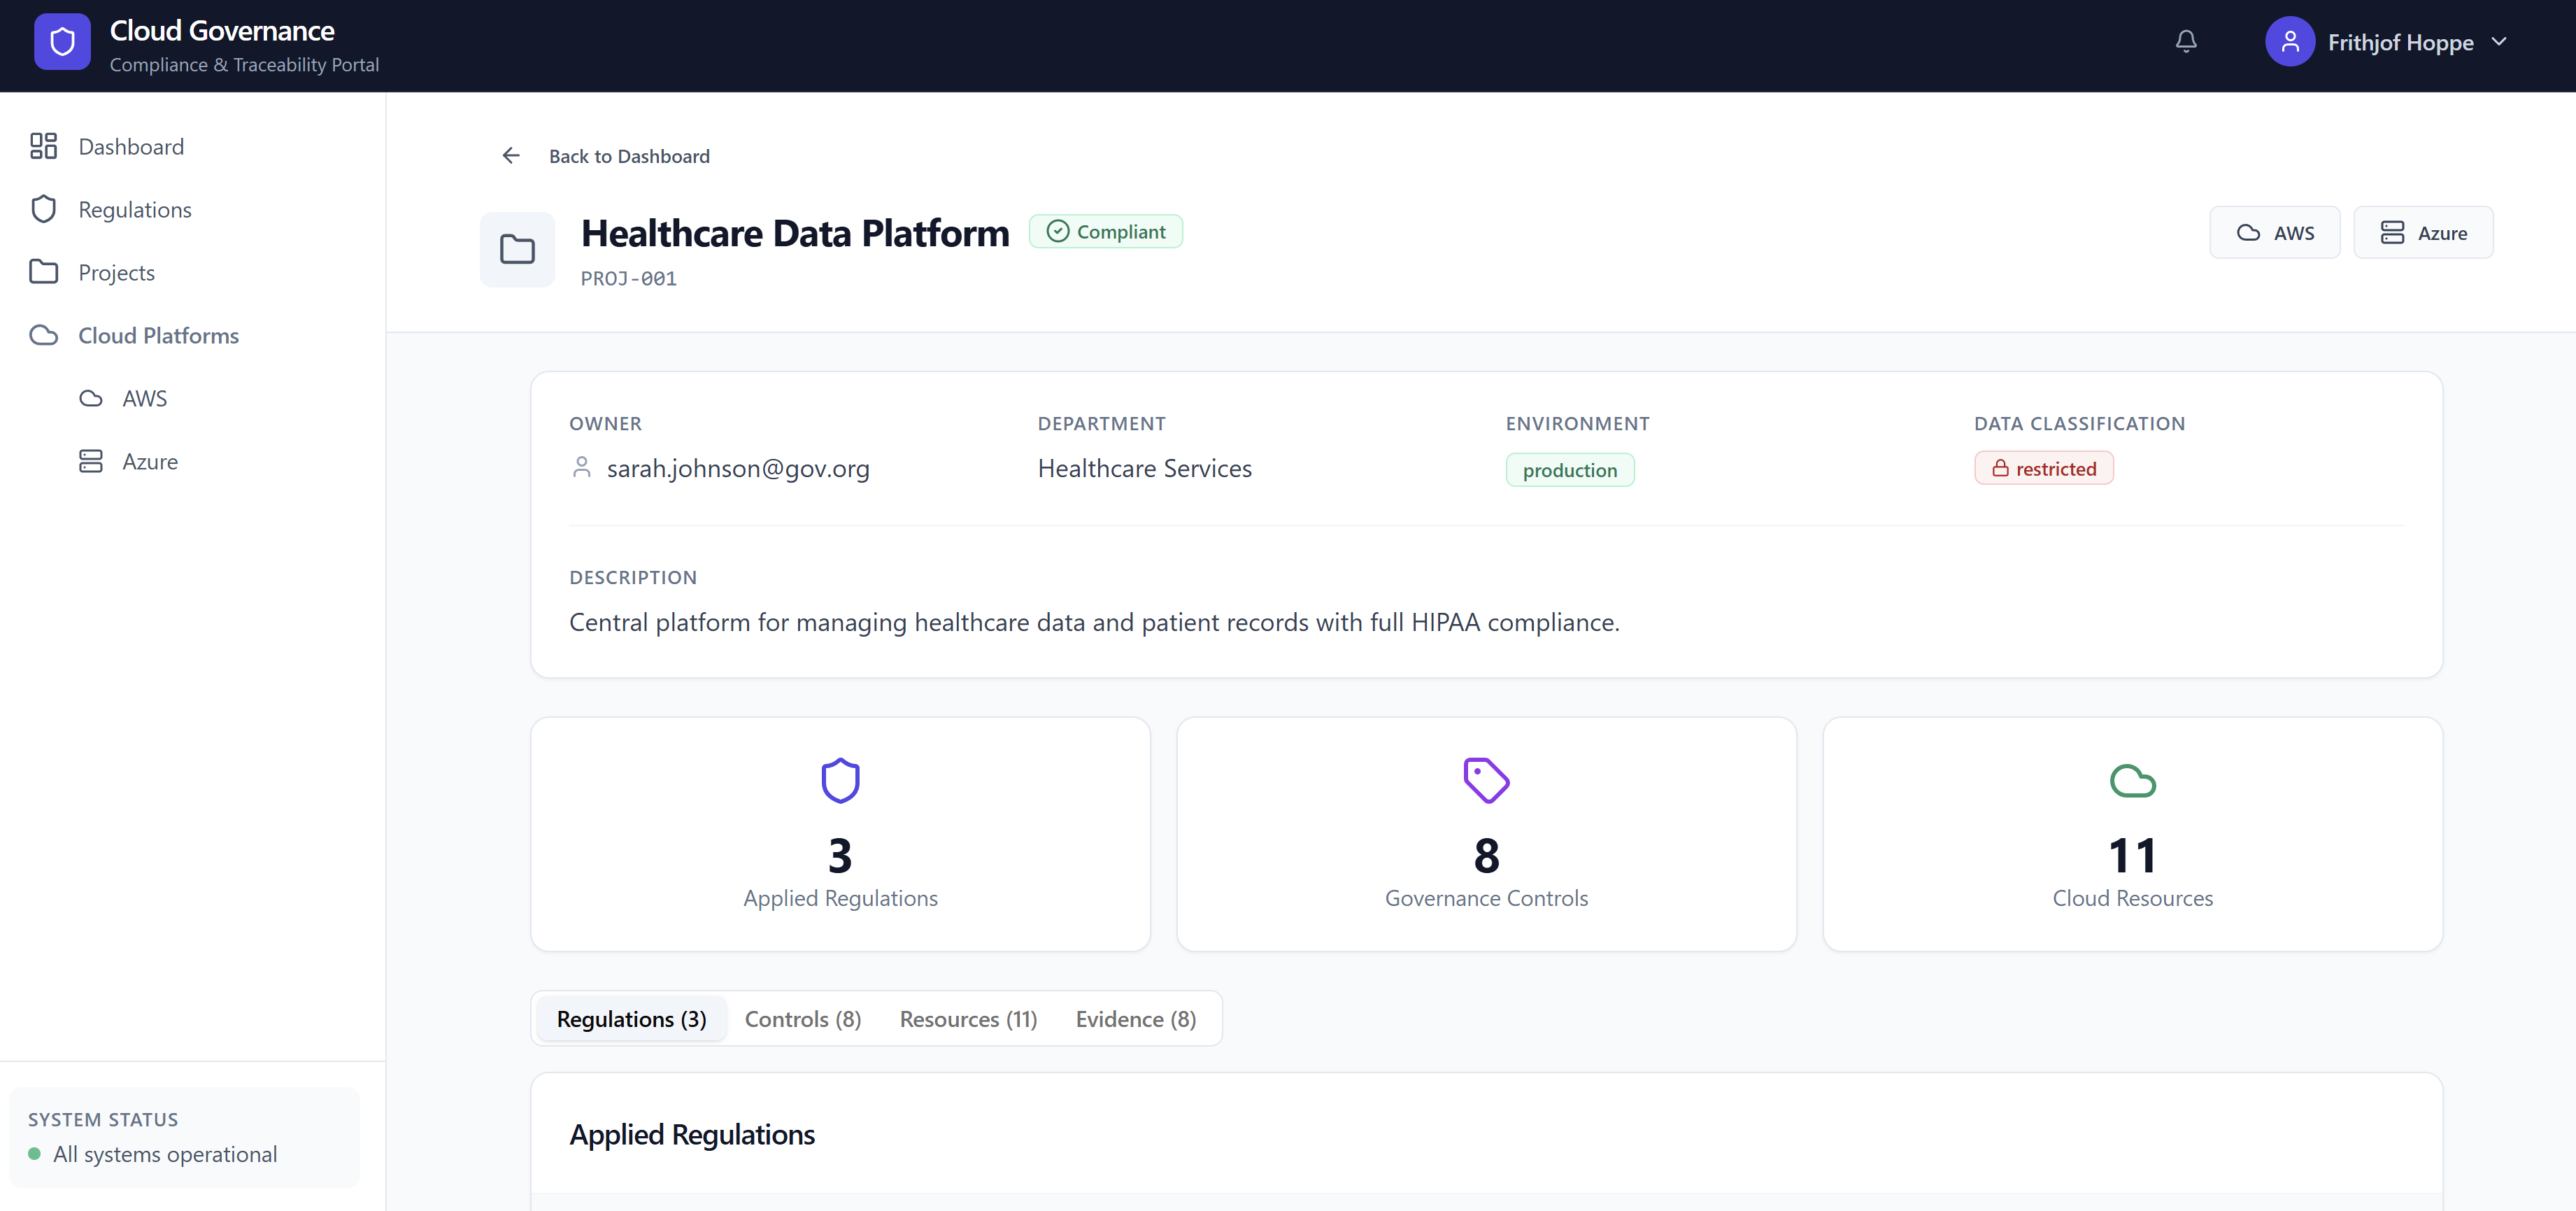
\includegraphics[width=0.8\textwidth]{graphics/ui-prototyp_project_healthcare.png}
    \caption{Detailansicht des Beispielprojekts Healthcare}
    \label{fig:methodology-project-healthcare-view}
\end{figure}

\begin{figure}[H]
    \centering
    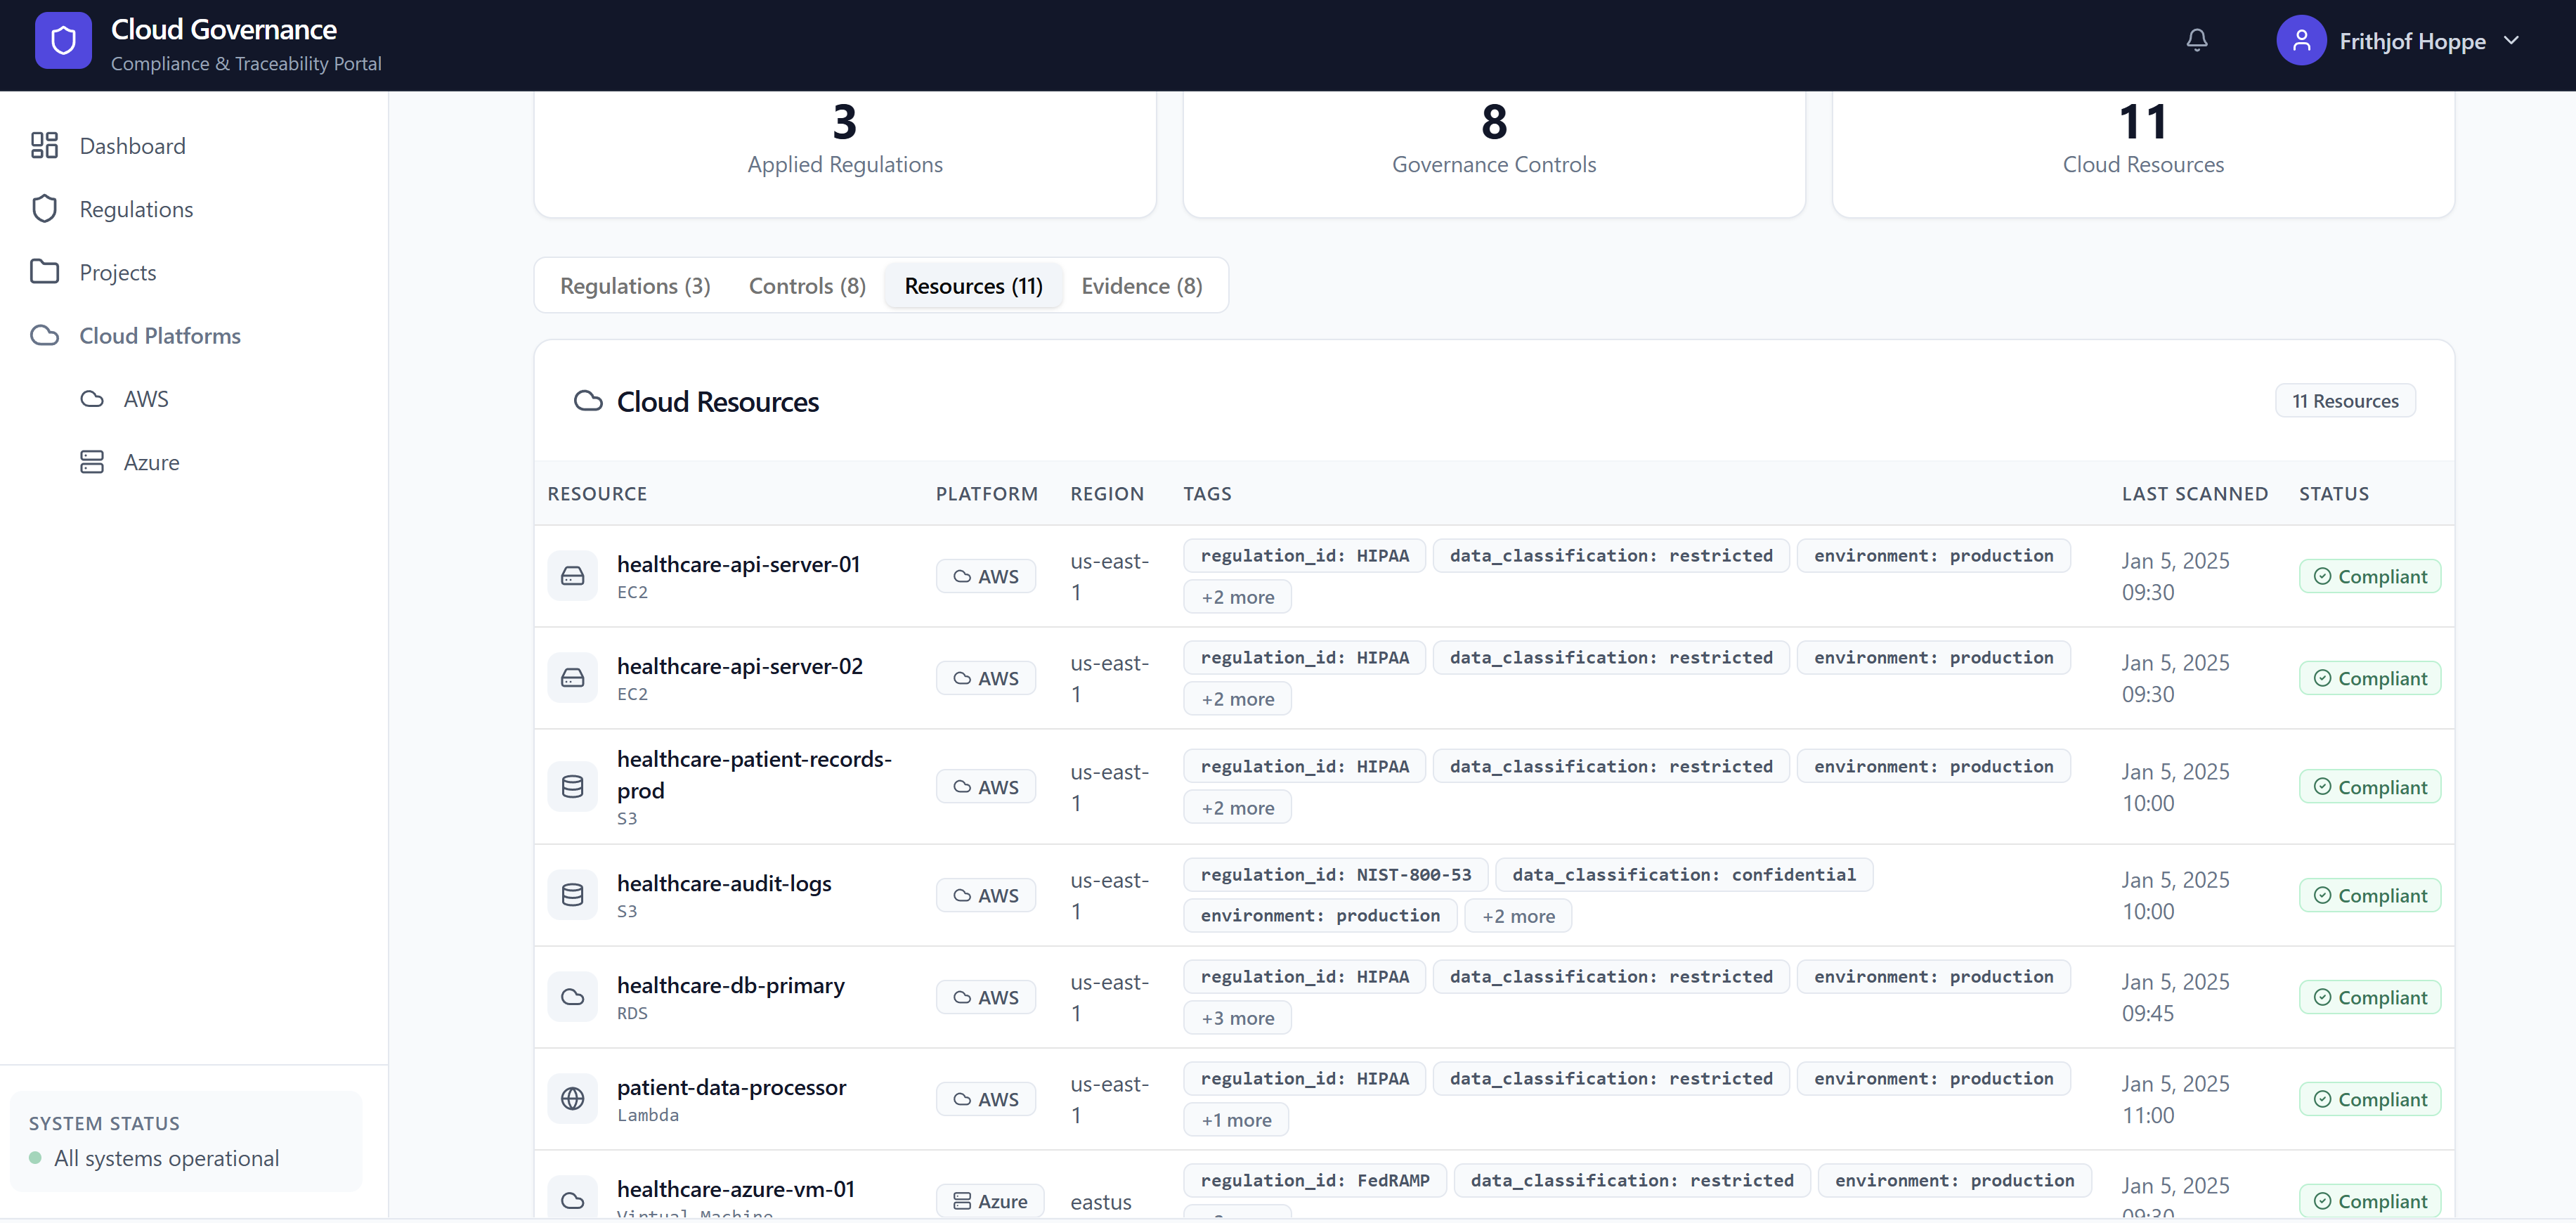
\includegraphics[width=0.8\textwidth]{graphics/ui-prototyp_project_healthcare_view_evidence.png}
    \caption{Detailansicht der beinhalteten Evidence im Beispielprojekt Healthcare}
    \label{fig:methodology-project-healthcare-view-evidence}
\end{figure}

Der \ac{poc} besteht aus den Komponenten in \autoref{fig:methodology-poc-setup}. Das 360-Grad-Cockpit verwaltet mit dem Project Service die Projekte inklusive der zugehörigen Foundations. Der \ac{lz} Provisioning Service provisioniert die Foundations auf den Cloud-Plattformen und hält Referenzen auf die erstellten Cloud Resource Container. Der Hauptanwender des 360-Grad-Cockpit ist der Projektverantwortliche. Das Governance Cockpit verawaltet mit dem Governance Configuration Service die Traceability-Relationship auf welcher Basis der Traceability Service Assessment vornimmt. Der Evidence Service speichert die Artefakte, welche den Stand der Compliance zu einem gewissen Zeitpunkt abbilden. Die Cloud Administration Komponenten provisioniert mit dem \ac{lz} Plattform Configuration Service die Grundinfrastruktur der \ac{lz}. Der Provisioning Service / IaC Execution Layer deckt die Interaktionen inkl. Provisionierung auf den Cloud-Plattformen da. Im \ac{poc} werden lediglich AWS und Azure repräsentativ für weitere grössere Cloud-Plattformen betrachtet.

Um den Fokus auf den genannten Use-Cases zu behalten wird in \autoref{fig:methodology-poc-setup} eine Auswahl getroffen welche Komponenten detailliert implementiert werden. Die grünen Komponenten werden detailliert umgesetzt, um die Funktionalität zu zeigen, die blauen Komponenten werden statisch implementiert da sie sich keinen direkten Bezug zur Funktionsweise der Traceability-Architecture aufweisen.

\begin{figure}[H]
    \centering
    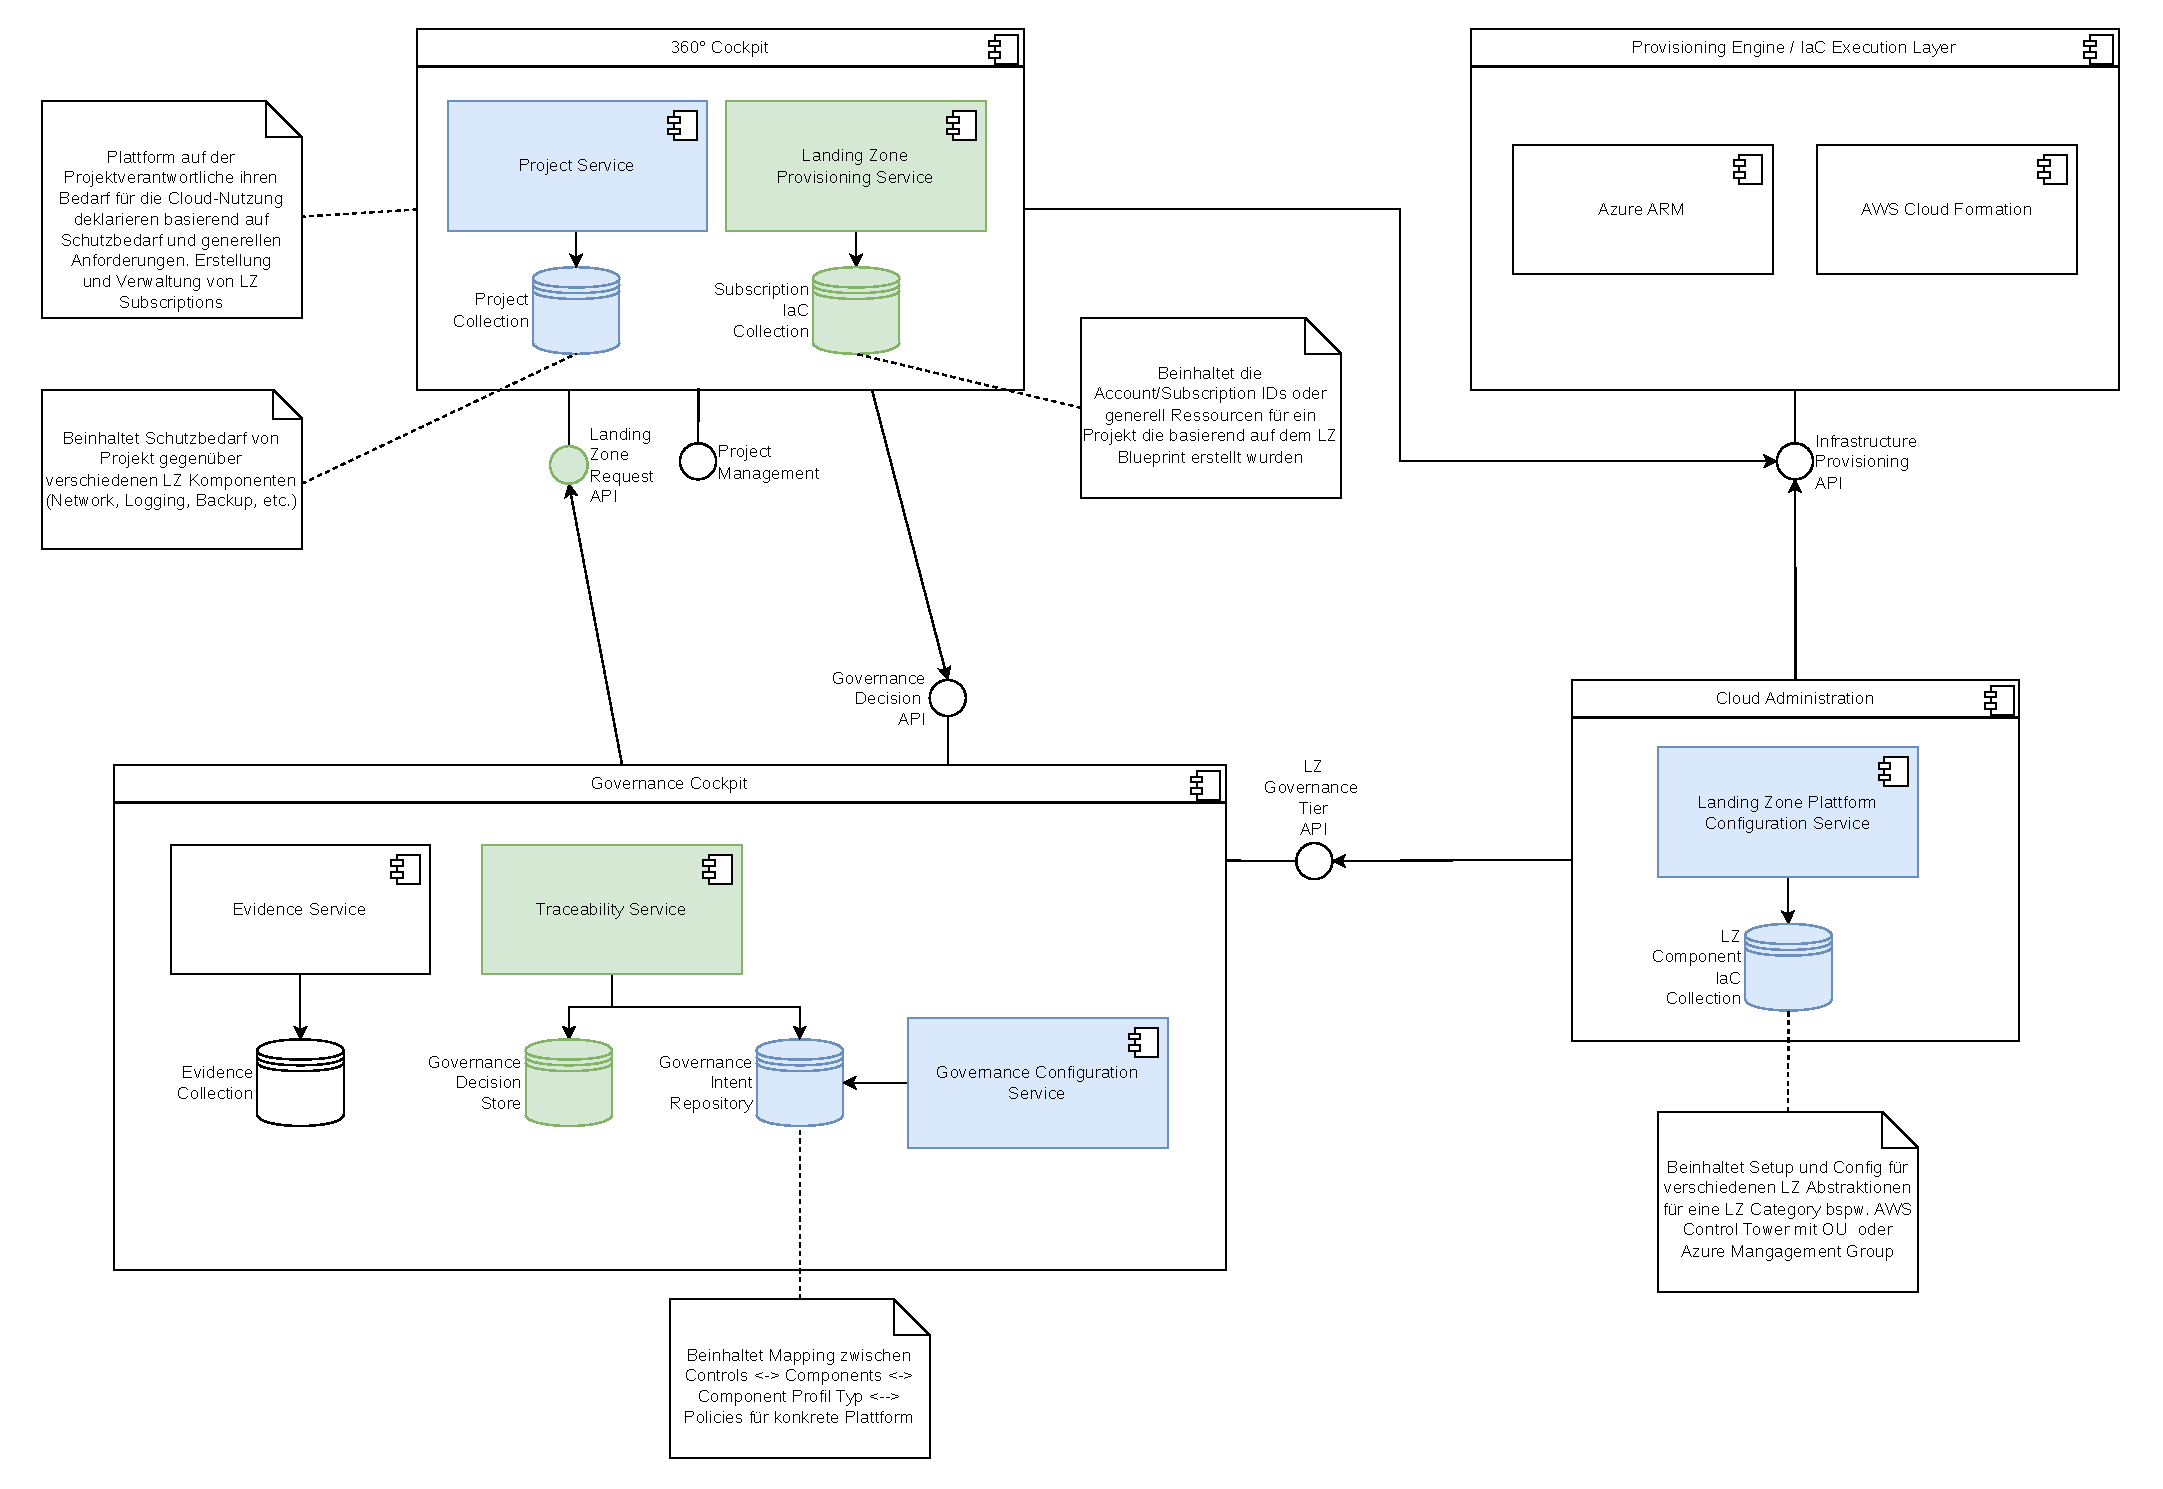
\includegraphics[width=\textwidth]{graphics/ip6-ideation-poc-components.drawio.pdf}
    \caption{Komponenten-Diagramm für den \ac{poc}}
    \label{fig:methodology-poc-setup}
\end{figure}

Im \ac{poc} ist für die Traceability der statisch konfigurierte Inhalte des Governance Configuration Service am relevantesten. Für die implementierte component-cenctric Variante werden in {fig:methodology-poc-traceability-relationship-components} dafür zuerst exemplarische Controls aus der Regulation \ac{si001} gewählt. Die Controls decken absichtlich unterschiedliche regulatorische Gebiete ab, damit eine Zuordnung zu verschiedenen Components in diesem Fall Storage, Network und Compute möglich ist. Nach den Controls werden bereits existieren Policies für die Cloud-Plattformen (Azure und AWS) mittels öffentlicher Dokumentation gesucht und wiederum Component/Component-Profiles zugewiesen. Die Component-Profiles werden im \ac{poc} nicht genauer spezifiziert und dienen lediglich als Veranschaulichung. Für eine produktive Anwendung müsste an dieser Stelle ein Security-Intent für ein Profil definiert werden und basierend auf diesem entsprechend Policies mit Parameter gemapped werden.

\begin{figure}[H]
    \centering
    \centering
    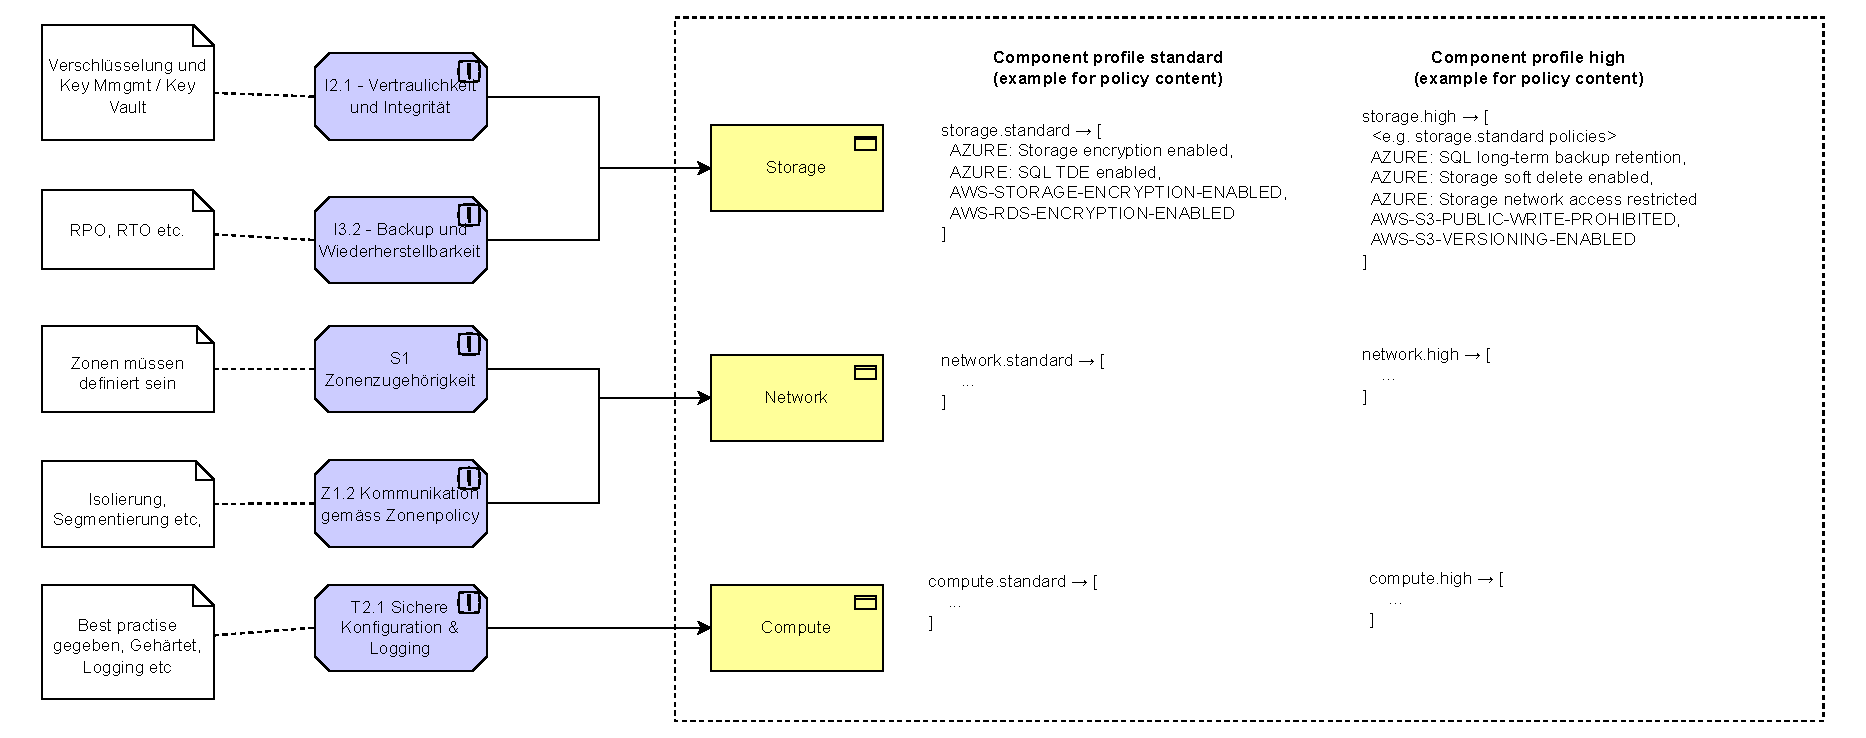
\includegraphics[width=\textwidth]{graphics/ip6-ideation-poc-traceability-components.drawio.pdf}
    \caption{Statische Traceability-Relationship Komponenten für den \ac{poc}}
    \label{fig:methodology-poc-traceability-relationship-components}
\end{figure}
\section{Traceability Architektur-Varianten}
\label{sec:traceability-architecture}

% \hl{structure notes start}
% \begin{itemize}
%     \item Basismodell / Subset vom Metamodell beschreiben auf welchen die Traceability Architektur aufbaut
%     \item Pro Architektur ein Kapitel, welche die Funktionsweise beschreibt und wie es gedenkt die Anforderungen zu erfüllen
% \end{itemize}
% \hl{structure notes end}

\subsection{Variante 1: Control-centric Bundling}
\label{sec:trace-arch-variant1}

\textbf{Ansatz}: Für jede Control in der jeweiligen Verordnung wird ein Mapping zu einem Plattform-Bundle gemacht. Also eine Control beinhaltet Plattform-Policies X, Y und Z. Beim Deployment einer \ac{lz} wählt das Blueprint aus welche Controls benötigt werden (z.B. keine Profile, erhöhter Schutzbedarf, etc.)

\textbf{Fokus}: Traceability

\textbf{Pros}
\begin{itemize}
    \item Rückverfolgbarkeit ist trivial: Das Ergebnis des Enforcements wird direkt einer Control-ID zugeordnet.
    \item Ideal für Audits (\flqq Zeig mir alle implementierten Controls\frqq).
\end{itemize}

\textbf{Cons}
\begin{itemize}
    \item Viele kleine Artefakte → erfordern Automatisierung und eine Build-Pipeline
    \item Einige Provider bevorzugen grössere Sets
\end{itemize}

\textbf{Fazit}: Diese Variante ist diejenige welche am besten die Traceability Anforderungen erfüllt, aber auch die aufwändigste in der Umsetzung ist. Es könnte als \flqq Goldstandard\frqq\ für die Traceability Architektur angesehen werden, aber es muss evaluiert werden ob der Aufwand gerechtfertigt ist im Vergleich zu den anderen Varianten.

\begin{figure}[H]
    \centering
    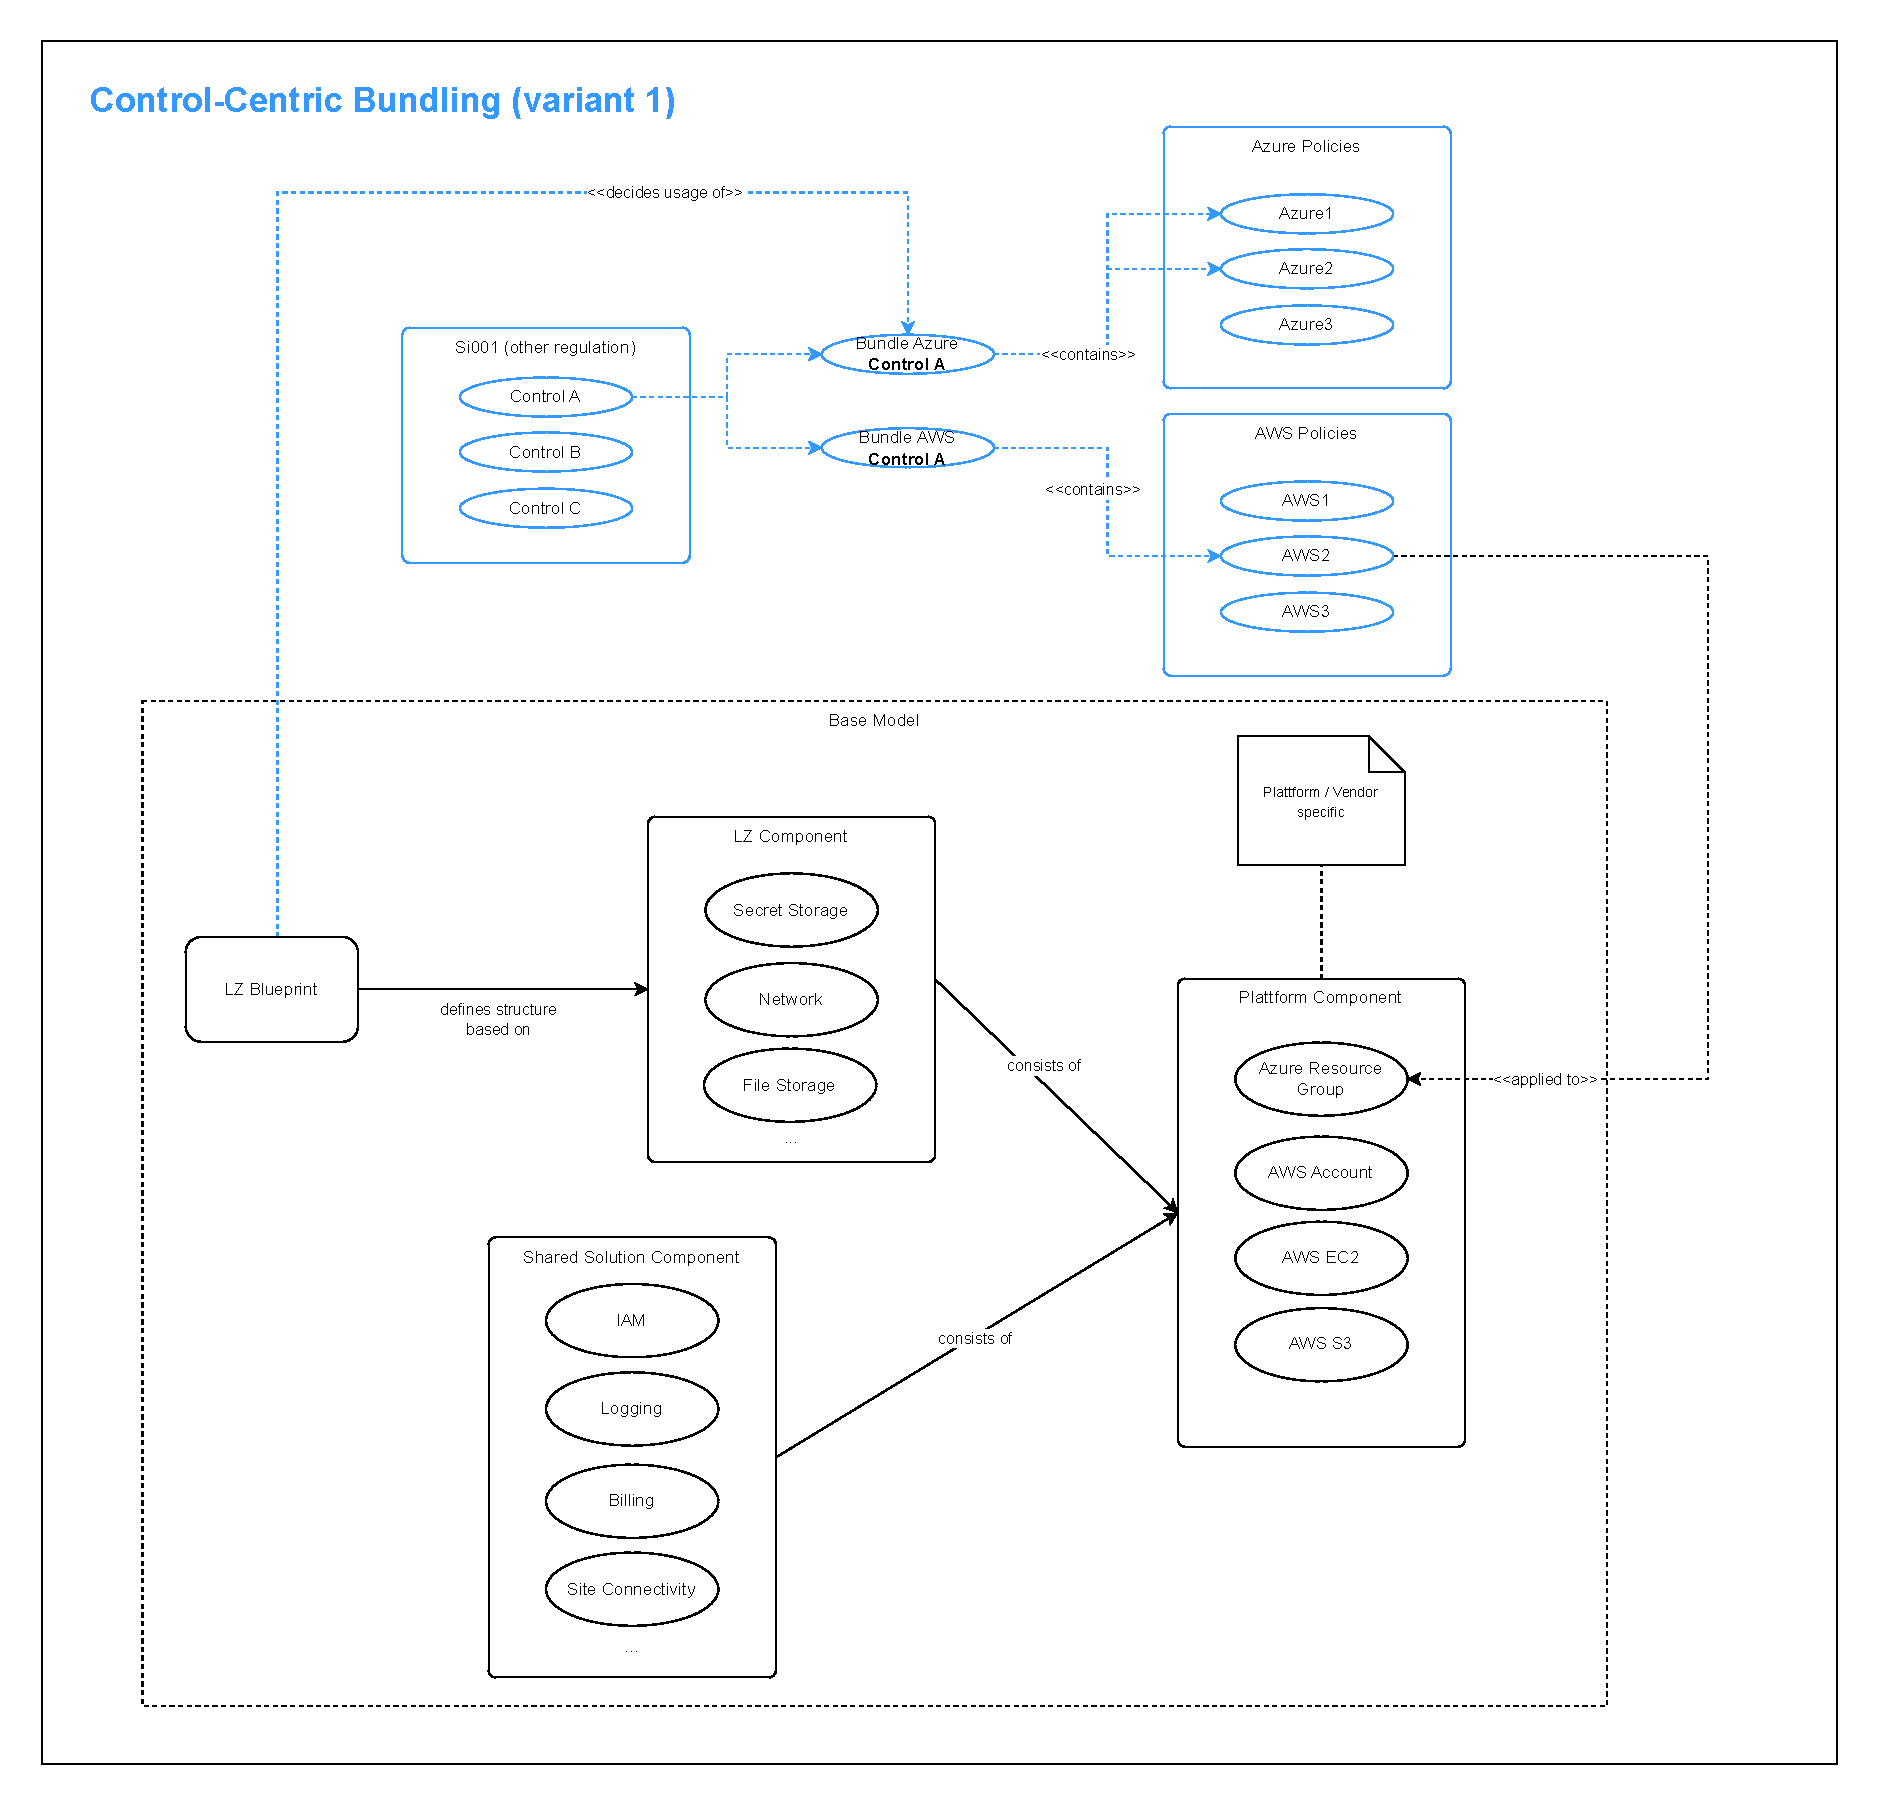
\includegraphics[width=\textwidth]{ip6-ideation-Traceability-Architecture-control-centric.drawio.pdf}
    \caption{Control-centric Traceability Architektur Variante}
    \label{fig:traceability-architecture-control-centric}
\end{figure}

\subsection{Variante 2: LZ component-centric Bundling}
\label{sec:trace-arch-variant2}

\textbf{Ansatz}: Die Controls werden nach \ac{lz}-Komponenten in Komponenten-Profiles gebündelt. Diese Profiles werden den Plattformrichtlinien zugeordnet. Bei der Bereitstellung einer \ac{lz} wählt der Blueprint die benötigten Komponenten und die Profiles der einzelnen Komponenten aus.

\textbf{Fokus}: Engineering, Verteilung an Expertengruppen/Teams, aber mit Rückverfolgbarkeit

Eine Regulation bildet ein Regelwerk wie z.B. \ac{si001} ab, welches die verschiedenen Controls enthält. Eine Control ist je eine Anforderung welche eingehalten werden muss damit die Control als eingehalten gilt.

\textbf{Funktionsweise}: Die Controls haben mind. eine Beziehung zu mind. einer \ac{lz}-Komponente, welche die Control implementiert. Für jede \ac{lz}-Komponente existieren verschiedene Profiles, diese Profiles bauen aufeinander auf, heisst die Nächsthöhere enthält Vorherige auch. Ein Profile kann jeweils mehrere Controls implementieren und bildet das Mapping zwischen Controls und konkreten Policies auf der jeweiligen Zielplattform. Policies können sowohl selbst definiert als auch vom Provider bereitgestellt sein.

\begin{figure}[H]
    \centering
    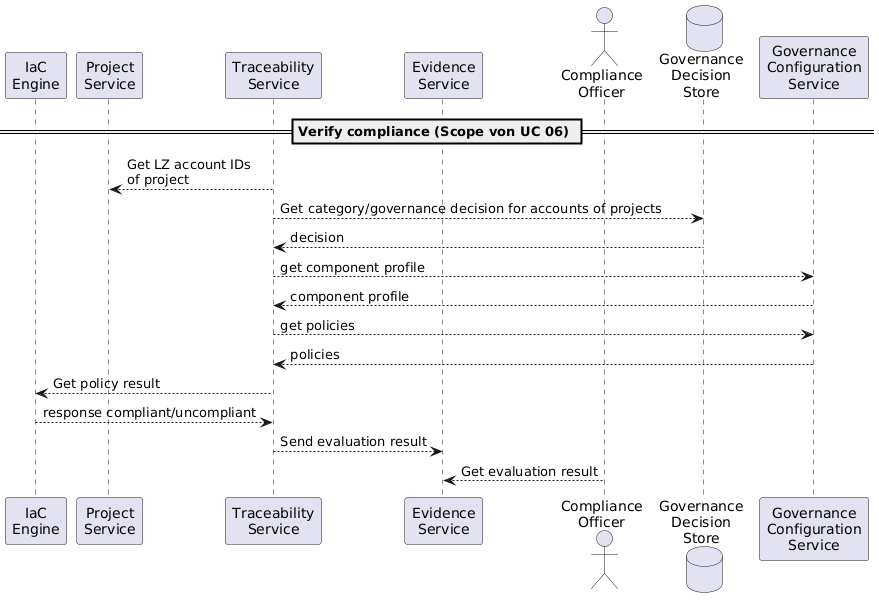
\includegraphics[width=\textwidth]{graphics/sequence-diagramm-poc_variant2_verify-compliance.png}
    \caption{Sequenz-Diagramm für Verifikation der Compliance nach Traceability Architektur Variante 2}
    \label{fig:methodology-poc-variant2-sequence-verification}
\end{figure}

\textbf{Pros}
\begin{itemize}
    \item Passt zur Implementierungspraxis von Teams: Netzwerkrichtlinien werden gemeinsam verwaltet
    \item Weniger Bundles, einfachere Einführung
\end{itemize}

\textbf{Cons}
\begin{itemize}
    \item Die Rückverfolgbarkeit erfordert einen zusätzlichen Suchschritt: \flqq Richtlinie X befindet sich im Bundle Netzwerk → enthält Controls A, B, C\frqq
    \item Einige Policies implementieren mehrere Controls (1:n)
\end{itemize}

\textbf{Fazit}: Diese Variante bietet einen guten Kompromiss zwischen Rückverfolgbarkeit und Praktikabilität, da sie die Implementierungspraxis der Teams berücksichtigt, aber dennoch eine gewisse Rückverfolgbarkeit ermöglicht. Es könnte als \flqq Silberstandard\frqq\ für die Traceability Architektur angesehen werden, da es eine praktikable Lösung darstellt, ohne den Aufwand der Control-zentrierten Variante zu erfordern.

\begin{figure}[H]
    \centering
    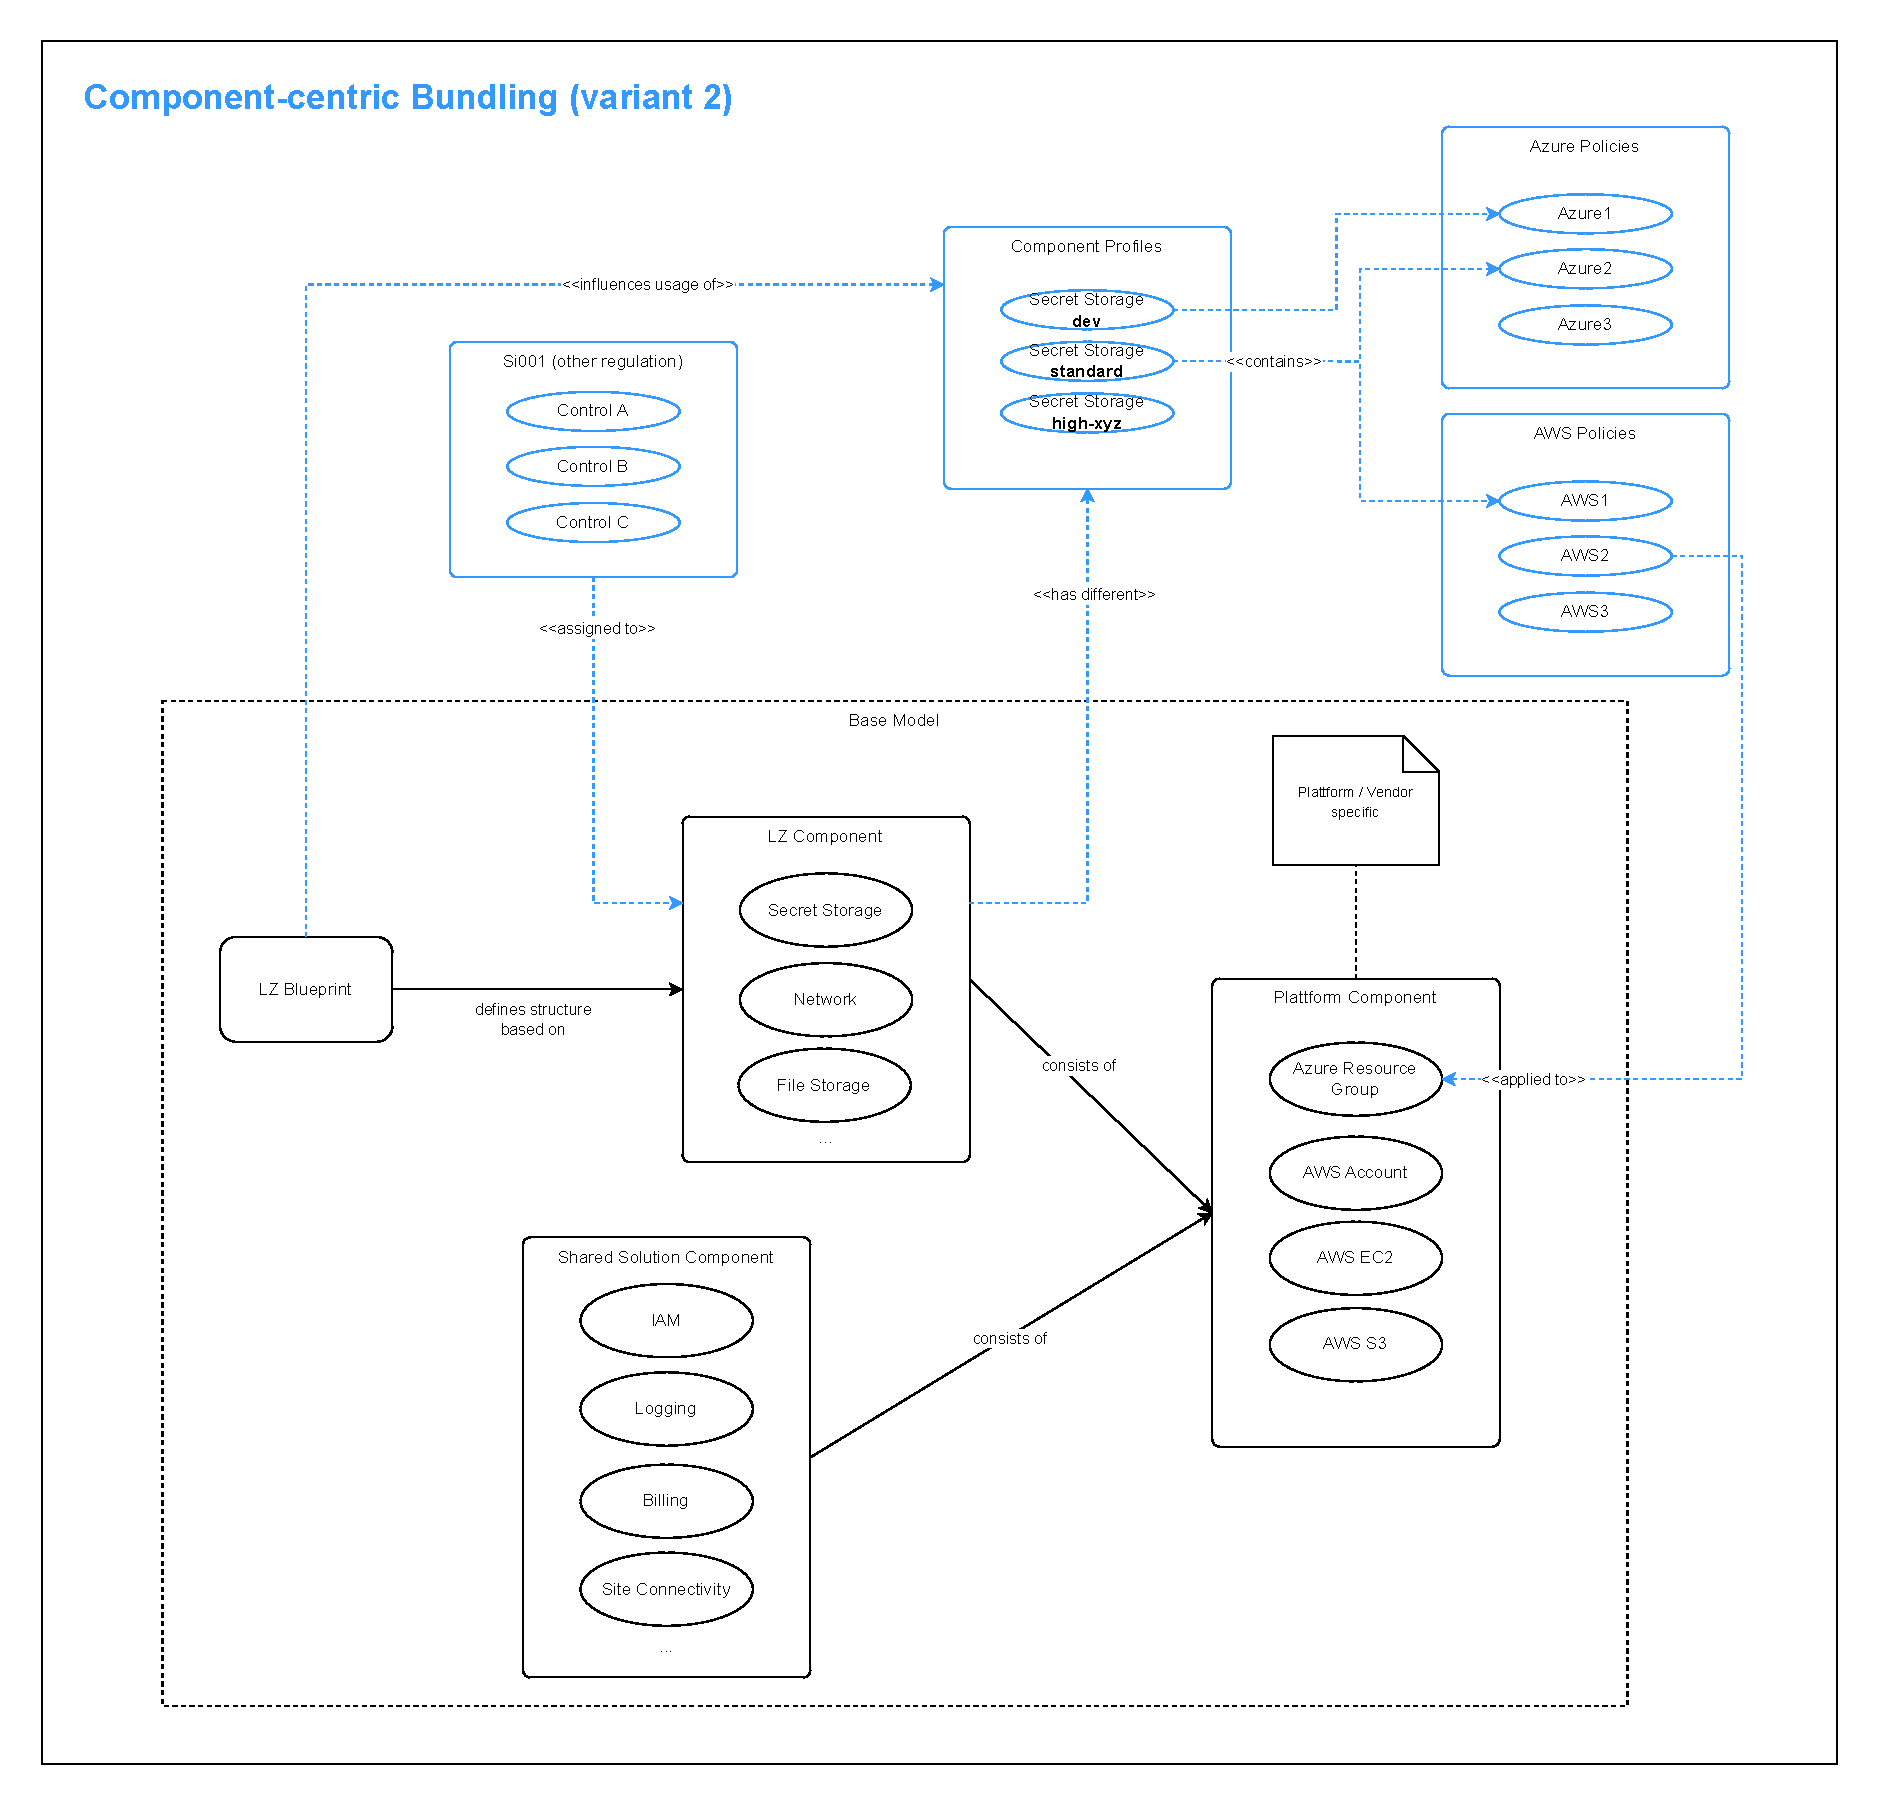
\includegraphics[width=\textwidth]{ip6-ideation-Traceability-Architecture-component-centric.drawio.pdf}
    \caption{Component-centric Traceability Architektur Variante}
    \label{fig:traceability-architecture-component-centric}
\end{figure}

\subsection{Variante 3: LZ category centric Bundling}
\label{sec:trace-arch-variant3}

\textbf{Ansatz}: Controls werden nach Profiles gebündelt, welche die Rules für alle Komponenten enthalten. Diese Profiles umfassen die entsprechenden Policies. Beim deployen einer \ac{lz} wählt der Blueprint nur die \ac{lz}-Profiles aus, der Rest wird abstrahiert.

\textbf{Fokus}: LZ-Kategorien mit Vereinfachung für den Endnutzer, da die Profile alles umfasst, ohne dass viel ausgewählt werden muss.

\textbf{Detailbeschreibung}: In dieser Architektur-Variante werden die Controls in Profiles gebündelt, die alle relevanten Regeln für die verschiedenen Komponenten enthalten. Jede Profile repräsentiert eine bestimmte \ac{lz}-Kategorie, die eine Risikoklasse oder einen Anwendungsfall abdeckt. Beim Deployen einer \ac{lz} wählt das Blueprint einfach die entsprechende Profile aus, ohne dass der Benutzer sich mit den einzelnen Controls oder Policies auseinandersetzen muss. Diese Herangehensweise bietet eine extrem einfache Anwendung und eine klare Customer Story, da die Kategorien direkt mit den Risikoklassen verknüpft sind. Allerdings führt dies zu einer hohen Duplikation von Controls über verschiedene Kategorien hinweg, und die Rückverfolgbarkeit zu einzelnen Controls erfordert die Pflege eines Manifests, das auflistet, welche Controls in welcher Profile enthalten sind.

\textbf{Pros}
\begin{itemize}
    \item Extrem einfache Anwendung (\flqq regulierte Profile anwenden\frqq)
    \item Klare Customer Story: Kategorien repräsentieren Risikoklassen
\end{itemize}

\textbf{Cons}
\begin{itemize}
    \item Hohe Duplikation von Controls über Kategorien hinweg
    \item Rückverfolgbarkeit zu einzelnen Controls ist gegeben, aber man muss ein Manifest \flqq Controls in der Profile\frqq\ führen
\end{itemize}

\textbf{Fazit}: Diese Variante bietet die einfachste Anwendung für den Endnutzer, da sie die Komplexität der Auswahl von Controls und Policies abstrahiert. Es könnte als \flqq Bronze-Standard\frqq\ für die Traceability Architektur angesehen werden, da es eine benutzerfreundliche Lösung darstellt, aber mit erheblichen Nachteilen in Bezug auf Duplikation und Rückverfolgbarkeit einhergeht.

\begin{figure}[H]
    \centering
    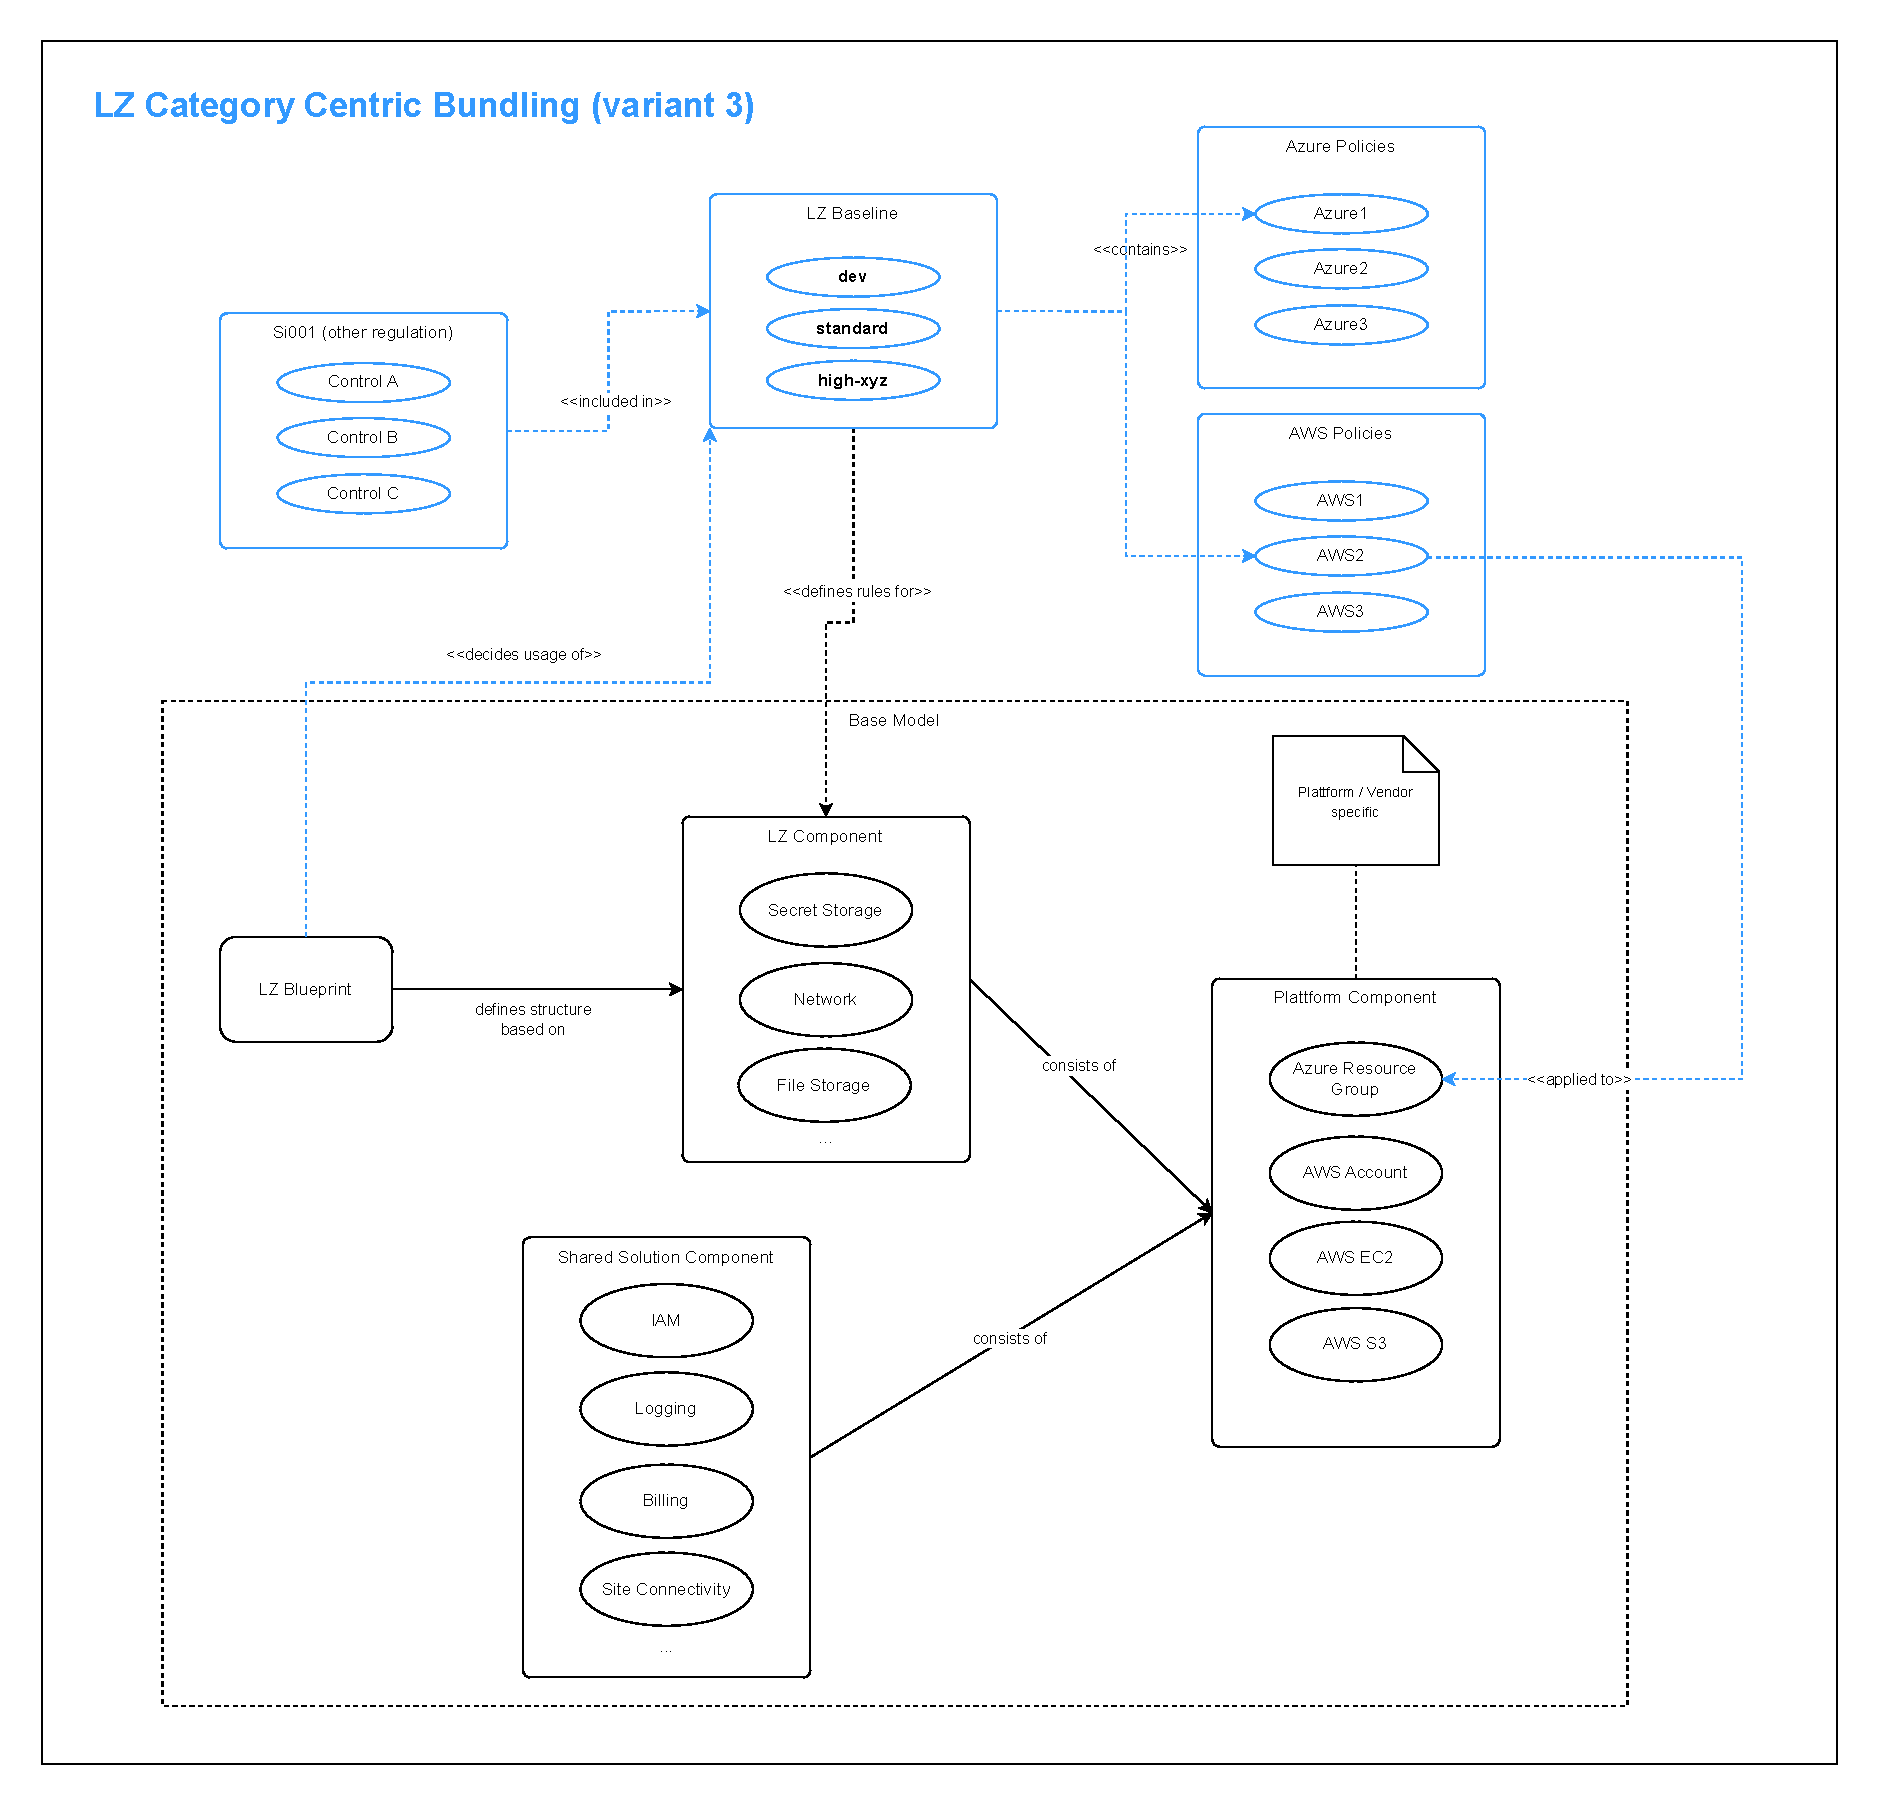
\includegraphics[width=\textwidth]{ip6-ideation-Traceability-Architecture-category-centric.drawio.pdf}
    \caption{LZ Category centric Traceability Architektur Variante}
    \label{fig:traceability-architecture-category-centric}
\end{figure}

\subsection{Variante 4: LZ Provider-native Bundling}
\label{sec:trace-arch-variant4}

\textbf{Ansatz}: Controls werden direkt durch die native Policy-Abstraction des Providers dargestellt (Azure Initiatives, AWS SCP usw.). Diese werden direkt auf die Komponenten angewendet.

\textbf{Fokus}: Die Anwendung von Richtlinien auf Ressourcen, weniger auf die Nachvollziehbarkeit (à la MVP). Initiativen/Bundles existieren bereits von verschiedenen Cloud-Providern.

\textbf{Detailbeschreibung}: In dieser Architektur-Variante werden die Controls direkt durch die nativen Richtlinienabstraktionen der Cloud-Provider dargestellt. Das bedeutet, dass die Implementierung der Controls direkt auf den Ressourcen erfolgt, ohne dass eine zusätzliche Abstraktionsschicht wie Bundles oder Profiles erforderlich ist. Diese Herangehensweise ermöglicht eine optimale Leistung und eine enge Ausrichtung an den Mechanismen der Provider, da sie die nativen Funktionen und Tools nutzt. Allerdings führt dies zu einer schlechteren Vergleichbarkeit über verschiedene Cloud-Provider hinweg, da jeder Provider unterschiedliche Formate und Strukturen für seine Richtlinien hat. Die Rückverfolgbarkeit erfordert daher eine Normalisierung über die verschiedenen Evidenceformate der Provider hinweg, um sicherzustellen, dass die Controls konsistent identifiziert und verfolgt werden können.

\textbf{Fazit}: Diese Variante bietet die beste Leistung und Providerausrichtung, da sie die nativen Mechanismen der Cloud-Provider nutzt. Es könnte als \flqq Performance-Standard\frqq\ für die Traceability Architektur angesehen werden, da sie die effizienteste Nutzung der Ressourcen ermöglicht, aber mit erheblichen Herausforderungen in Bezug auf Vergleichbarkeit und Rückverfolgbarkeit einhergeht.

\textbf{Pros}
\begin{itemize}
    \item Operativ sauber: Nutzung der nativen Mechanismen der Provider
    \item Beste Leistung und Providerausrichtung
\end{itemize}

\textbf{Cons}
\begin{itemize}
    \item Cloud-übergreifende Vergleichbarkeit wird schlechter
    \item Traceability muss über verschiedene Evidenceformate der Provider hinweg normalisiert werden
\end{itemize}

\begin{figure}[H]
    \centering
    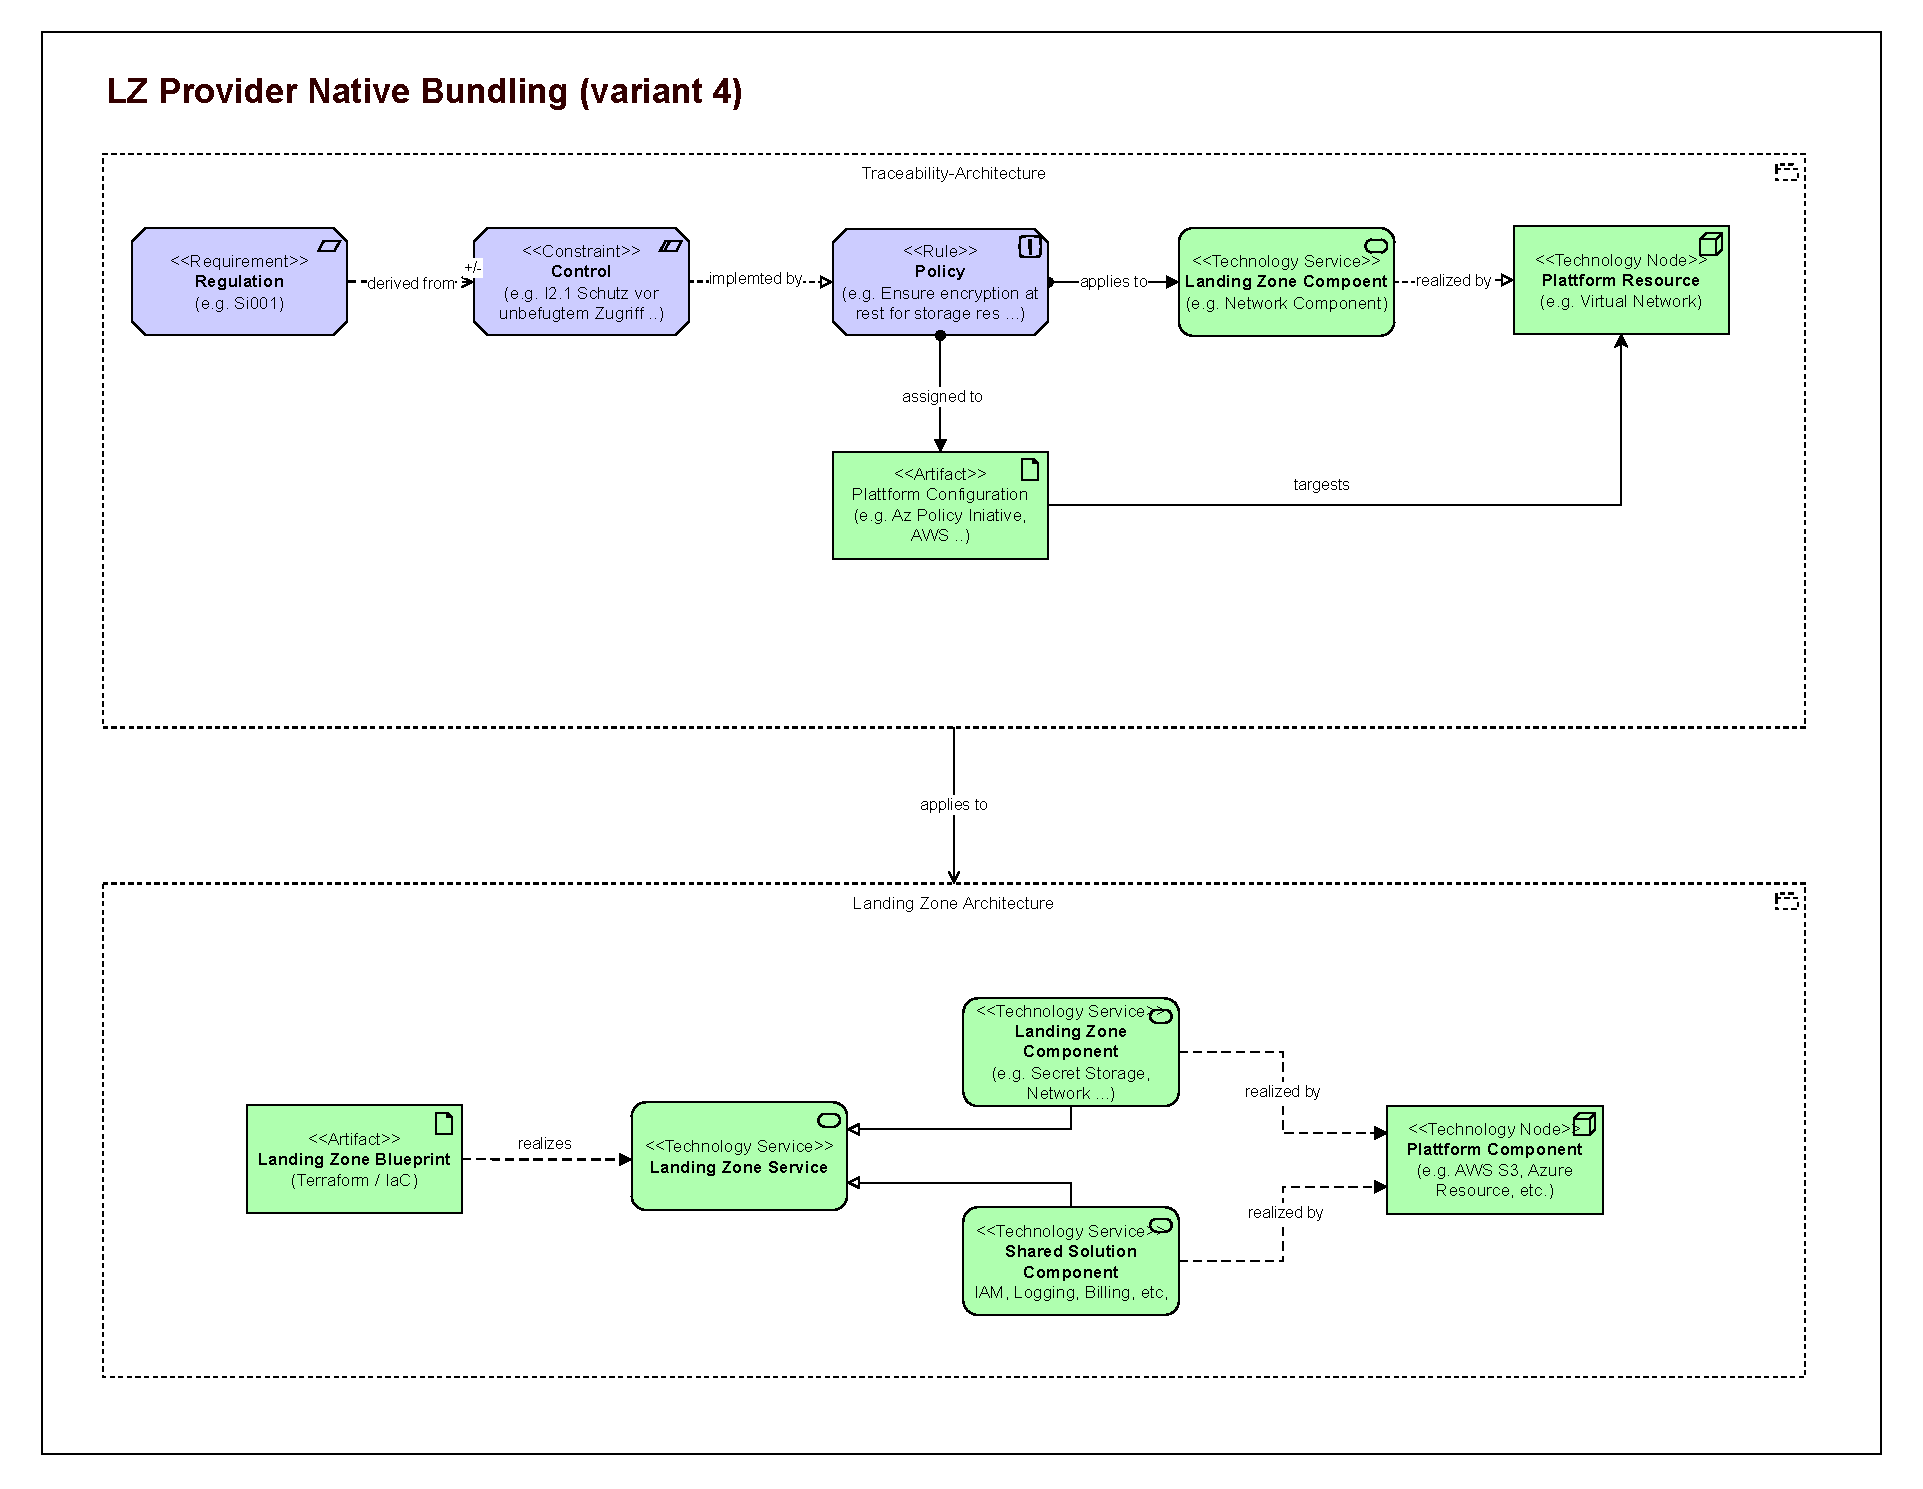
\includegraphics[width=\textwidth]{ip6-ideation-Traceability-Architecture-provider-native.drawio.pdf}
    \caption{LZ Provider Native Traceability Architektur Variante}
    \label{fig:traceability-architecture-provider-native}
\end{figure}
\section{Umsetzung des Proof of Concept}
\label{sec:umsetzung}

Technisch werden das 360°-Cockpit sowie das Governance-Cockpit mittels einer Python Anwendung mit FastAPI implementiert. Die Nutzung des Python Setups begründet sich damit, dass die CLIs von Anbietern wie Azure und AWS auf Python basieren. Des Weiteren ermöglicht FastAPI mit vergleichbar geringem Aufwand einen RESTful Service zu erstellen. Um die Trennung der beiden Cockpit Komponenten zu betonen, passieren gegenseitige Aufrufe jeweils via HTTP Interface. Zur Persistierung verwenden die Komponenten Project Collection, Evidence Collection, Governance Decision Store und Governance Intent Repository eine MongoDB Document Database. Die Wahl einer Document Database begründet sich mit der Abbildung der Traceability-Beziehung als JSON-Objekte, was eine Handhabung aus implementatorischer Sicht vereinfacht. Für den Landing Zone Plattform Configuration Service wird ein statisches IaC Setup mit Terraform verwendet. Die modellierten Traceability-Beziehungen werden hierbei als statischer Inhalt geteilt. Über das Setup hinaus werden weitere Cloud-Ressourcen erzeugt welche in einem funktionalen Setup bereits als gegeben angenommen werden:

\begin{itemize}
    \item Techinsche Benutzer / Service Accounts für die automatisierte wie manuelle Provisionerung von Cloud-Ressourcen
    \item Verrechnungsstruktur als Vorraussetzung zur Erzeugung von Subscriptions/Accounts
    \item Initiale Subcriptions/Accounts für Komponentn welche über verschiedenen Landing-Zones hinweg verwendet werden (bspw. Analytics Workspace)
\end{itemize}

Die Traceability-Beziehungen werden basierend auf dem Basismodell in \fullref{sec:trace-arch-variant2} modelliert und im Rahmen der Umsetzung adaptiert. Für den Scope im \ac{poc} wird 

\begin{figure}[H]
    \centering
    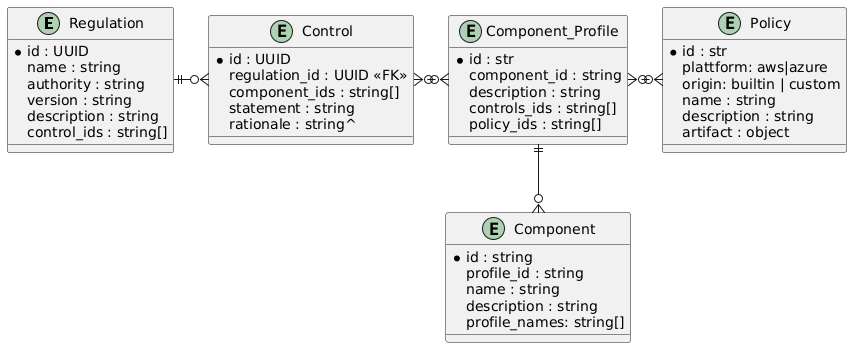
\includegraphics[width=\textwidth]{graphics/poc_data_model.png}
    \caption{Datenmodell für Traceability-Beziehung im \ac{poc}}
    \label{fig:data-model-poc}
\end{figure}


% @startuml
% entity "Regulation" as regulation {
%   *id : UUID
%   name : string
%   authority : string
%   version : string
%   description : string
%   control_ids : string[]
% }

% entity "Control" as control {
%   *id : UUID
%   regulation_id : UUID <<FK>>
%   component_ids : string[]
%   statement : string
%   rationale : string^
% }

% entity "Policy" as policy {
%   *id : str
%   plattform: aws|azure
%   origin: builtin | custom
%   name : string
%   description : string
%   artifact : object
% }

% entity "Component_Profile" as component_profile {
%   *id : str
%   component_id : string
%   description : string
%   controls_ids : string[]
%   policy_ids : string[]
% }

% entity "Component" as component {
%   *id : string
%   profile_id : string 
%   name : string
%   description : string 
%   profile_names: string[]
% }


% regulation ||-right-o{ control
% component_profile ||--o{ component
% control }o-right-o{ component_profile
% policy }o-left-o{ component_profile
% @enduml
\section{Evaluation}
\label{sec:evaluation}

\hl{stucture start}
\begin{itemize}
    \item Evaluation ob sich die Bewertung der Variante bewahrheitet hat. Wurden die Kriterien wie erwartet erfüllt? Findings?
    \item Evaluation der nicht implementierten Varianten mit der Erfahrung von den implementierten Varianten
    \item Zusammenfassung welche Variante am optimalsten ist für den Use-Case vom BIT
\end{itemize}
\hl{structure end}

\section{Diskussion}
\label{sec:discussion}

5.1 Interpretation of the Findings
•	Significance of the identified similarities 
•	Significance of the identified differences 
•	Assessment of the extent to which landing zone can be treated as a common cross-provider concept 
5.2 Value of a Common Definition
•	Usefulness of a shared definition for technical comparison 
•	Relevance for architecture, governance, and multi-cloud discussions 
5.3 Limitations of the Comparative Result
•	Remaining ambiguity caused by provider-specific terminology and scope 
•	Limits of conceptual comparison without practical validation 

\section{Abschluss}
\label{sec:abschluss}

\subsection{Zusammenfassung der Ergebnisse}

\begin{itemize}
    \item Rekapitulation der Zielsetzung der Arbeit
    \item Synthese der zentralen Erkenntnisse aus Architekturkonzeption, Proof of Concept und Evaluation
    \item Gesamtbewertung der untersuchten Architekturvarianten
\end{itemize}

\subsection{Beantwortung der Forschungsfragen}

\begin{itemize}
    \item Explizite Beantwortung der Forschungsfragen auf Basis der erzielten Ergebnisse
    \item Einordnung der wichtigsten Architekturprinzipien für strukturierte Landing-Zone-Architekturen
\end{itemize}

\subsection{Beitrag der Arbeit}

\begin{itemize}
    \item Konzeptioneller Beitrag zur Strukturierung von Landing-Zone-Architekturen im EA-Kontext
    \item Methodischer Beitrag zur Bewertung von Architekturvarianten
    \item Praktischer Beitrag durch Umsetzung eines Proof of Concept
\end{itemize}

\subsection{Ausblick}

\begin{itemize}
    \item Weiterführende Evaluation weiterer Capabilities
    \item Anwendung des Ansatzes in realen Transformationsprojekten
    \item Untersuchung organisatorischer und wirtschaftlicher Auswirkungen
    \item Weiterentwicklung von Tooling zur Architektur-Governance
\end{itemize}
\section{Hilfsmittel}
\label{sec:hilfsmittel}

\begin{table}[H]
    \centering
    \begin{tabularx}{\textwidth}{|p{3.4cm}|X|p{4.5cm}|}
        \hline
        \textbf{Hilfsmittel} & \textbf{Verwendung} & \textbf{Betroffene Stellen} \\
        \hline
        Elicit.ai & Recherche von Literatur für die Erarbeitung der Grundlagen \& Darstellung des Kapitels & \fullref{sec:grundlagen}
        \\
        \hline
    \end{tabularx}
    \caption{verwendete Hilfsmittel}
    \label{tab:hilfsmittel}
\end{table}

%%---BIBLIOGRAPHY------------------------------------------------------------------------

{\sloppypar
\printbibliography[heading=bibintoc, title=Quellenverzeichnis]
}
\clearpage
\printglossary[type=\acronymtype]


%%---APPENDIX----------------------------------------------------------------------------
\include{sections/eigenstaendigkeit}
\selectlanguage{ngerman}				%ngerman or english
% \include{sections/authenticity}
% \selectlanguage{enlish}				%ngerman or english
\begin{appendix}

\section{Example appendix}
\label{appendix:ui-mockup}


%%---NOTES for DEBUG---------------------------------------------------------------------
%\newpage
%\listoftodos[\section{Todo-Notes}]
%\clearpage

\end{document}